
\newcommand{\nomedoc}{Analisi Dei Requisiti}
\newcommand{\versione}{1.7}
\newcommand{\versioneglossario}{2.0}
\newcommand{\versionenormeprogetto}{2.0}
\newcommand{\nomefile}{AnalisiDeiRequisiti-\versione.pdf}
\newcommand{\datacreazione}{2 Dicembre 2010}
\newcommand{\datamodifica}{29 Gennaio 2011}
\newcommand{\stato}{formale}
\newcommand{\uso}{esterno}
\newcommand{\redazione}{Baron Federico\\&Daminato Simone}
\newcommand{\verifica}{Caputo Cosimo}
\newcommand{\approvazione}{Lovato Daniele}
\newcommand{\distribuzione}{
VT.G \\
& Prof. Vardanega Tullio\\
& Prof. Cardin Riccardo }

% FUNZIONI TIPOGRAFICHE
\newcommand{\co}{\texttt} % courier
\newcommand{\bo}{\textbf} % bold
\newcommand{\pr}{\par\medskip} % paragrafo spaziato
\newcommand{\sca}{\textsc} % small caps

\documentclass[a4paper,12pt]{report}
% 10pt,11pt,12pt
% titlepage, notitlepage -> per dare inizio o no ad una nuova pagina dopo titolo
% twoside -> per dire se fronte-retro
\usepackage[latin1]{inputenc}
% per caratteri accentati
\usepackage[italian]{babel}
% per regole sintattiche italiane
\usepackage[bookmarks=true, pdfborder={0 0 0 0}]{hyperref}
% per collegamenti ipertestuali
\usepackage{graphicx}
% per inserimento immagini

% \usepackage{enumerate}
% per personalizzare elenchi puntati

\usepackage[hmargin=2cm]{geometry} %margine 2 cm
%\geometry{options varie}

% comandi per gestire meglio header e footer
\usepackage{fancyhdr}  % header e footer
\usepackage{totpages}
\pagestyle{fancy}
\renewcommand{\headrulewidth}{0.4pt}
\renewcommand{\footrulewidth}{0.4pt}

\setlength{\headheight}{1.2cm} % NON TOCCARE
\setlength{\voffset}{-1.5cm} % NON TOCCARE
\setlength{\textheight}{666pt} % NON TOCCARE
\setlength{\footskip}{60pt}
\setlength{\parindent}{0pt} % INDENTAZIONE

\lhead{\nomedoc\  (ver. \versione)}
\chead{}
\rhead{
\includegraphics[height=1cm]{img/netmus.png}}
\lfoot{
\includegraphics[height=0.8cm]{img/logo.png}}
\cfoot{}
\rfoot{\thepage}

\usepackage{titlesec}
\titleformat{\chapter}{\normalfont\huge\bfseries}
{\thechapter}{20pt}{\Huge}

\usepackage{rotating}   % PER TABELLE E AMBIENTI RUOTATI
\usepackage{array}
\usepackage{color}
\usepackage{colortbl}  % VARIE PER GESTIRE I COLORI
\definecolor{Orange}{RGB}{255,127,0}   % ARANCIO ACCES0
\definecolor{orange}{RGB}{255,207,80}  % ARANCIO TENUE

\addtocontents{toc}{\protect\thispagestyle{fancy}}  % PER INDICI CON + PAGINE
\usepackage[font=it]{caption}    % PER RENDERE CORSIVE LE DIDASCALIE
\usepackage{eurosym}  % PER SIMBOLO EURO

% \usepackage{listings}   per codice sorgente

\author{VT.G - Valter Texas Group}

\begin{document}

\pagenumbering{Roman} % INIZIO NUMERAZIONE ARABA

\vspace*{1cm}
\begin{center}

\begin{LARGE} \sca{Federico Baron} \end{LARGE}\\
\vspace{0.5cm}
\begin{Large}
\emph{fede.baron.89@gmail.com} \end{Large}\\
\vspace*{1cm} 
\includegraphics[width=5cm]{img/logo.png}\\
\vspace{0.5cm}
\begin{Large} \emph{``Comunicazione Aumentata/Alternativa per Giovani Ospiti
della Terapia Intensiva Pediatrica''} \end{Large}\\
\vspace{3cm}
\begin{Large} \sca{\nomedoc} \end{Large}\\
\end{center}
\vspace{1cm}

% INFORMAZIONI DOCUMENTO
\begin{center}
\begin{tabular}{r|l}
\hline & \\
\bo{Nome} & \nomefile \\
\bo{Versione attuale} & \versione \\
\bo{Data creazione} & \datacreazione \\
\bo{Data ultima modifica} & \datamodifica \\
\bo{Redazione} & \redazione \\
& \\\hline
\end{tabular}
\end{center}
\newpage

% REGISTRO MODIFICHE
\section*{Registro delle modifiche}

\begin{longtable}{|p{0.13\textwidth}|c|p{0.2\textwidth}|p{0.46\textwidth}|}
\hline
\rowcolor{orange} \bo{Data} & \bo{Versione} & \bo{Autore} & \bo{Descrizione} \\
\hline
\endhead
\hline
\endfoot
\hline
29/01/2011 & 1.7 & Palazzin Alberto & Correzione di errori grammaticali e
semantici in tutto il documento. Correzione a fronte della verifica di qualit\`a
dei requisiti.
\\
\hline
\hline
23/01/2011 & 1.6 & Baron Federico & Aggiornamento del tracciamento con i nuovi
codici degli use-cases. Leggera modifica dei capitoli 2.4 e 2.5.
\\
\hline
21/01/2011 & 1.5 & Mandolo Andrea & Corretti Riferimenti.
\\
\hline
17/01/2011 & 1.4 & Baron Federico & Eliminazione di UC2.2 e modifica della
gerarchia degli use-case con assegnamento di nuovi codici
identificativi.
\\
\hline
15/01/2011 & 1.3 & Caputo Cosimo & Modifica di tutte le immagini (.png)
relative ai diagrammi use-case in seguito a cambio di tecnologia utilizzata.
\\
\hline
14/01/2011 & 1.2 & Baron Federico & Corretti UC1 e UC1.1 secondo le
indicazioni proposte nella valutazione di RR. UC1 \`e stato diviso in UC1A e
UC1B. \\
\hline
12/01/2011 & 1.1 & Mandolo Andrea & Modificato layout Registro delle
modifiche.\\
\hline
19/12/2010 & 1.0 & Lovato Daniele & Validazione per consegna RR.\\
\hline
18/12/2010 & 0.11 & Caputo Cosimo & Verificato l'intero documento.\\
\hline
17/12/2010 & 0.10 & Daminato Simone & Inserite tabelle per il tracciamento dei
requisiti, liste di immagini e tabelle.\\
\hline
17/12/2010 & 0.9 & Daminato Simone & Inserimento dell'use case, diagramma e
testo, UC3.\\
\hline
 15/12/2010 & 0.8 & Baron Federico & Aggiunta del capitolo ``Sommario''.
 Correzione di alcuni errori grammaticali. Inserite tabelle in LateX del C1.\\
\hline
14/12/2010 & 0.7 & Baron Federico & Inserimento degli use case, diagrammi e
testo, UC1, UC1.1, UC2, UC2.1, UC 2.2.\\
\hline
 13/12/2010 & 0.6 & Baron Federico & Indicizzazione e reinserimento tabelle,
inserimento della figura 1 (Diagramma architetturale).\\
\hline
13/12/2010 & 0.5 & Baron Federico & Inserimento tabelle dei requisiti
riassuntive per C1.\\
\hline
13/12/2010 & 0.4 & Daminato Simone & Stesura completa dell'elenco dei requisiti
della Componente 2.\\
\hline
13/12/2010 & 0.3 & Baron Federico & Stesura completa dell'elenco dei requisiti
della Componente 1.\\
\hline
09/12/2010 & 0.2 & Daminato Simone & Redazione del capitolo 2.\\
\hline
07/12/2010 & 0.1 & Lovato Daniele & Redazione del capitolo 1.\\
\end{longtable}


% INDICE
\tableofcontents

\chapter*{Sommario}
Nel presente documento vengono individuati ed elencati i requisiti che VT.G si
propone di soddisfare nello sviluppo del software richiesto dal capitolato
d'appalto C02 NetMus. Per favorire la comprensione dell'analisi proposta sono
descritti alcuni diagrammi use-case che rispettano lo standard \underline{UML}
2.0 e deducono la quasi totalit\`a dei requisiti elaborati.
Nel presentare questa Analisi dei Requisiti si \`e scelto di separare
chiaramente le due componenti fondamentali, quella di invio dati e quella di persistenza e
visualizzazione, che costituiscono il sistema NetMus e che dovranno essere il
pi\`u possibile indipendenti.

\thispagestyle{fancy} % serve perche' nelle pagine di inizio Chapter esca header e footer
\pagenumbering{arabic} % INIZIO NUMERAZIONE NORMALE
\rfoot{\thepage\ di \pageref{TotPages}}
\addcontentsline{toc}{chapter}{Sommario}

\chapter{Introduzione}
\thispagestyle{fancy} % serve perche' nelle pagine di inizio Chapter esca header e footer

\section{Scopo del documento}
Il presente documento ha lo scopo di presentare al committente l'Analisi dei
Requisiti e le potenzialit\`a del nostro prodotto software per soddisfare le
richieste del capitolato d'appalto C02 NetMus (vedi 1.4.2 - Riferimenti
Normativi).


\section{Scopo del prodotto}
Il progetto \underline{NetMus} nasce con lo scopo di realizzare un sistema
software basato su \underline{cloud} \underline{computing}, per memorizzare
informazioni di brani musicali in profili utente online.\\ Tali informazioni vengono estratte da
dispositivi musicali o di archiviazione \underline{USB} al momento della loro connessione.

\section{Glossario}
Il Glossario \`e definito con un documento a parte
(\emph{Glossario-\versioneglossario.pdf}). Tutti i termini caratterizzati da
\underline{questa sottolineatura} sono ivi definiti.\\
Verr\`a sottolineata solamente la prima occorrenza di ciascun
termine presente nel Glossario, per non compromettere la leggibilit\`a del documento.

\section{Riferimenti}

\subsection{Normativi} % oppure rif. a Norme di progetto con leggi e tutto
\begin{itemize}
  \item ISO/IEC 12207:1995 - Cicli di vita software
  \item ISO/IEC 9126:2001 - Quality Model
  \item \emph{NormeDiProgetto-\versionenormeprogetto.pdf} che regola e
  accompagna tutti i documenti ufficiali.
\end{itemize}
\newpage
\subsection{Informativi}
\begin{itemize}
  \item Capitolato d'appalto CO2-NETMUS del corso di Ingegneria del Software
  A.A. 2010/11 :\\
  \url{http://www.math.unipd.it/~tullio/IS-1/2010/Progetto/NetMus.pdf}
  \item Slide delle lezioni del corso:\\
  \url{http://www.math.unipd.it/~tullio/IS-1/2010/}
  \item Verbale intervista proponente:\\
  \co{allegato Verbale-1.0.pdf}
  \item Sistema di cloud Google App Engine:\\
  \url{http://code.google.com/intl/it/appengine/}
\end{itemize}


% INIZIO CAPITOLO 2
\chapter{Descrizione generale}
\thispagestyle{fancy}

\section{Contesto d'uso del prodotto}
Il progetto NetMus che abbiamo intenzione di sviluppare \`e un software
destinato ad una vasta gamma d'utenza, con et\`a maggiore o uguale
a 12 anni, ma in particolare adolescenti e adulti dai 15 ai 35 anni.

\subsection{Piattaforma d'esecuzione e interfacciamento con l'ambiente di
installazione e uso}
Il prodotto finale utilizzer\`a diverse tecnologie (in particolare:
\underline{Java}, \underline{GAE}, \underline{GWT} e \underline{JavaFX}) che
renderanno possibile l'utilizzo del sistema su pi\`u piattaforme d'esecuzione con sistemi operativi diversi, i cui unici due requisiti
fondamentali saranno di possedere una connessione ad \underline{Internet} e di aver
installata una Java Runtime Environment non obsoleta (JRE 6 Update 13 minimo).
In particolare, il prodotto finale sar\`a testato sui principali sistemi operativi: \underline{Windows} (xp e 7), \underline{Linux} (principali e
pi\`u diffuse distribuzioni), \underline{Mac OS X} (Snow Leopard).
\section{Funzioni del prodotto}
Il prodotto finale sar\`a composto da due componenti. Una componente di
persistenza e visualizzazione della libreria virtuale dell'utente. Un'altra
componente di recupero delle informazioni dei brani musicali contenuti nei
sistemi di riproduzione personale dell'utente. La prima componente avr\`a il
compito di gestire la memorizzazione delle informazioni dei brani nel database,
di visualizzazione e di gestione tramite un'interfaccia semplice e facilmente
utilizzabile. La seconda componente svolger\`a il ruolo di estrazione delle
informazioni dai brani musicali e le invier\`a al server senza interferire con
l'utente che intanto potr\`a continuare a svolgere il proprio lavoro
indisturbato. L'estrazione avverr\`a non appena verr\`a rilevato un nuovo
dispositivo di archiviazione di massa (storage USB o lettore mp3)
che non cripta i propri file, e in modo del tutto autonomo verranno ricavate le
informazioni, memorizzate in locale e successivamente inviate al server.

\section{Caratteristiche degli utenti}
L'utente tipo che utilizza il sistema non \`e in possesso di particolari
conoscenze informatiche, ma \`e in grado di navigare sul web e di eseguire alcune
semplici operazioni correlate (come per esempio effettuare un login).

\section{Vincoli generali}
Il software nel suo funzionamento e sviluppo:
\begin{itemize}
  \item sar\`a completo della documentazione necessaria e del manuale d'uso;
  \item sar\`a portabile (verr\`a testato e garantito il suo funzionamento sui
  principali sistemi operativi);
  \item sar\`a sicuro per gli utenti (garantir\`a il controllo del proprio
  account, dei propri dati e della propria privacy);
  \item la visualizzazione e l'utilizzo avverranno tramite browser (sar\`a
  necessaria la connessione ad Internet);
  \item il manuale utente sar\`a fornito sia in italiano che in inglese.
\end{itemize}

\section{Assunzioni e dipendenze}
Si assume che sui personal computer utilizzati dagli utenti sia gi\`a installata
una \underline{JVM} che non sia ad una versione obsoleta. Sar\`a
necessaria l'installazione di una JRE  versione 6 update 13 minimo.

\section{Glossario}
Esister\`a un unico glossario comune a tutti i documenti, contenente la
spiegazione di tutti i termini e gli acronimi che verranno utilizzati
all'interno della documentazione. Questo documento sar\`a organizzato in ordine
alfabetico in modo da permettere una rapida ricerca dei termini e sar\`a suddiviso
due categorie: termini e acronimi.

\chapter{Diagramma architetturale}
\thispagestyle{fancy}
Per facilitare la comprensione degli use case si fornisce un diagramma
architetturale che rappresenta ad altissimo livello come sar\`a strutturato
l'intero sistema NetMus. Si evidenzia la concomitanza tra le due componenti fondamentali
del sistema, quella di persistenza e visualizzazione (C1) e quella di
recupero delle informazioni (C2).
\vspace{1cm}

\begin{figure}[h]
  \centering
  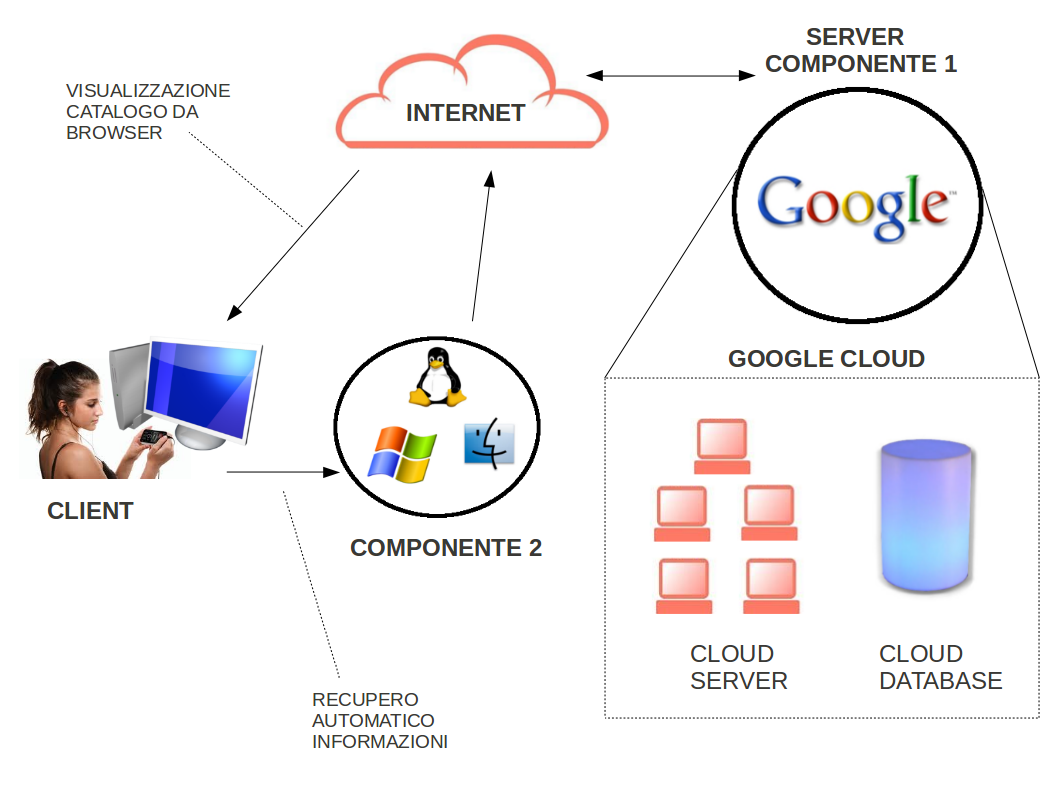
\includegraphics[width=16cm]{img/AR/DiagrammaArchitetturale.png}
\caption{Diagramma architetturale che descrive ad altissimo livello la
struttura delle interazioni che l'utente avr\`a con il sistema NetMus. }
\end{figure}

\chapter{Use case}
\thispagestyle{fancy}

\section{UC1 - Sistema NetMus, componente di persistenza e visualizzazione}

\begin{figure}[h]
  \centering
  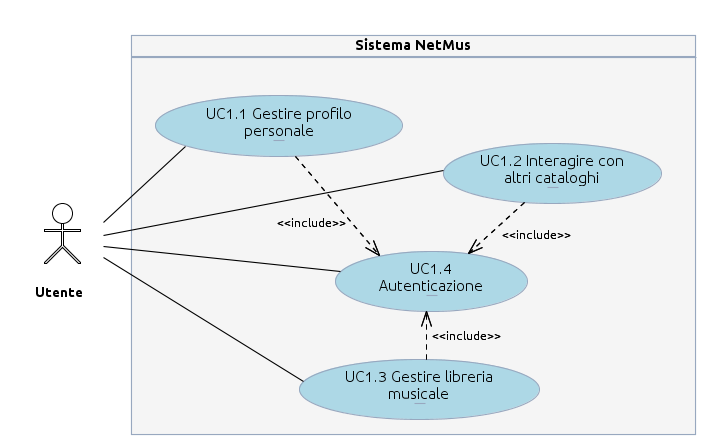
\includegraphics[width=14.5cm]{img/AR/UC1.png}
\caption{Diagramma dei casi d'uso che descrive le principali funzionalit\`a della
componente di persistenza e visualizzazione.}
\end{figure}

\vspace*{0.5cm}
\bo{Use case UC1: Sistema NetMus, componente di persistenza e visualizzazione}\\\\ 
\bo{Attori primari:} Utente. \\\\
\bo{Pre-condizioni:} Il portale \`e attivo e l'utente, connesso ad internet, vi
accede tramite un browser. \\\\ 
\bo{Post-condizioni:} Il portale NetMus \`e attivo, ha soddisfatto tutte le
richieste dell'utente ed \`e pronto a soddisfarne altre. \\\\ 
\bo{Scenario principale:} 
\begin{enumerate}
  \item L'utente effettua l'autenticazione (UC1.4).
  \item L'utente, tramite browser, fa un certo numero di richieste tra quelle
  possibili per visualizzare o modificare informazioni al sistema (UC1.1, UC1.2
  e UC1.3 in qualsiasi ordine).
  \item Le richieste dell'utente vengono tutte soddisfatte in un tempo
  accettabile.
\end{enumerate}
\bo{Scenari secondari:}
\begin{itemize}
  \item La comunicazione tra utente e NetMus fallisce per un problema di
  connessione.
  \begin {enumerate}
    \item Non c'\`e possibilit\`a di procedere fino a quando la connessione sar\`a
    ristabilita. I dati che erano stati aggiornati prima del verificarsi del
    problema sono gi\`a stati salvati.
  \end{enumerate}
\end{itemize}
\newpage

\section{UC2 - Sistema NetMus, componente di recupero delle informazioni}

\begin{figure}[h]
  \centering
  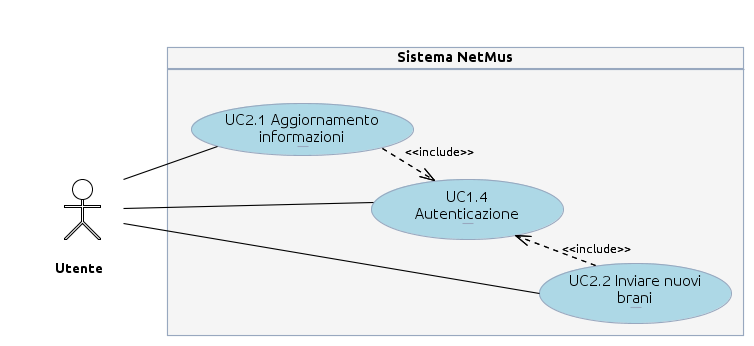
\includegraphics[width=15cm]{img/AR/UC2.png}
\caption{Diagramma dei casi d'uso che descrive le principali funzionalit\`a della
componente di recupero delle informazioni.}
\end{figure}

\vspace*{0.5cm}
\bo{Use case UC2: Sistema NetMus, componente di recupero delle informazioni}\\\\
\bo{Attori primari:} Utente \\\\
\bo{Pre-condizioni:} Il portale \`e attivo e l'utente, connesso ad internet, vi
accede tramite un browser. \\\\ 
\bo{Post-condizioni:} Online sono state inviate al server tutte le
informazioni riguardanti nuovi brani musicali presenti nel computer o altre periferiche
dell'utente. I dati dei file musicali dell'utente sono stati aggiornati con
informazioni aggiuntive reperite da NetMus. Il sistema \`e pronto a ricevere altre
richieste per l'invio o l'aggiornamento di informazioni. \\\\
\bo{Scenario principale:} 
\begin{enumerate}
  \item L'utente effettua l'autenticazione (UC1.4).
  \item Vengono inviate a NetMus tutte le nuove informazioni recuperate (UC2.2).
  \item I brani dell'utente vengono aggiornati con eventuali informazioni
  aggiuntive reperite da NetMus (UC2.1).
\end{enumerate}
\bo{Scenari secondari:}
\begin{itemize}
  \item La comunicazione fallisce per un problema di connessione, oppure si
  accede alla componente 2 in modalit\`a offline.
  \begin {enumerate}
    \item L' invio (UC2.2) prosegue registrando tutte le nuove informazioni
    in locale in modo che siano pronte non appena venga stabilita una
    connessione.
    \item L'aggiornamento dei brani dell'utente (UC2.1) non pu\`o avere luogo.
  \end{enumerate}
\end{itemize}
\newpage

\section{UC1.4 - Autenticazione}
\begin{figure}[h]
  \centering
  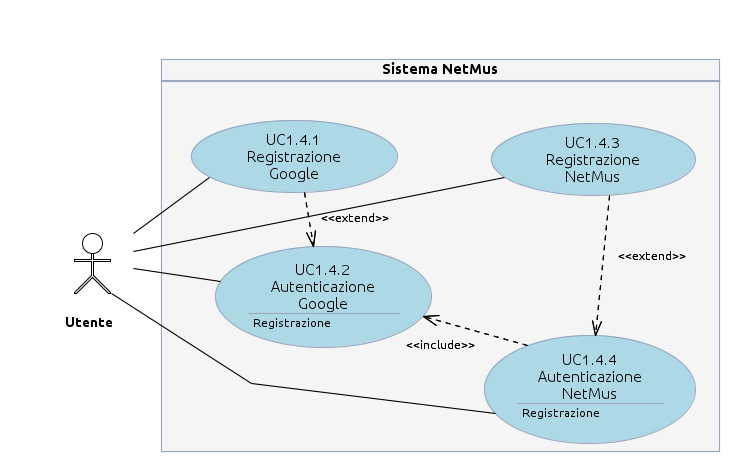
\includegraphics[width=15cm]{img/AR/UC1_4.png}
\caption{Diagramma dei casi d'uso che descrive la procedura di autenticazione
del sistema NetMus.}
\end{figure}

\vspace{1cm}
\bo{Use case UC1.4: Autenticazione}\\\\
\bo{Attori primari:} Utente. \\\\
\bo{Pre-condizioni:} Il portale \`e attivo e l'utente, connesso ad Internet, vi
accede tramite un browser. \\\\
\bo{Post-condizioni:} L'utente \`e autenticato e tutte le funzionalit\`a di
NetMus sono funzionanti e disponibili. \\\\
\bo{Scenario principale:} 
\begin{enumerate}
  \item L'utente inserisce dei dati di login validi (UC1.4.3).
  \item Netmus verifica i dati ed autentica l'utente.
\end{enumerate}
\bo{Scenari secondari:}
\begin{itemize}
  \item L'utente inserisce dei dati di login non validi (UC1.4.3).
  \begin {enumerate}
    \item Il tentativo di autenticazione fallisce.
    \item L'utente non \`e in grado di accedere a NetMus, pu\`o decidere di
    riprovare l'autenticazione (UC1.4.3) o effettuare la registrazione
    (UC1.4.2).
  \end{enumerate}
  \item L'utente decide di effettuare la registrazione (UC1.4.2).
  \begin {enumerate}
    \item L'utente esegue i passi standard per la registrazione a NetMus
    (UC1.4.2).
    \item L'utente ora possiede i dati necessari per effettuare l'autenticazione (UC1.4.3, UC1.4.1).
  \end{enumerate}
\end{itemize}
\newpage


\section{UC1.1 - Gestione del profilo personale}
\begin{figure}[h]
  \centering
  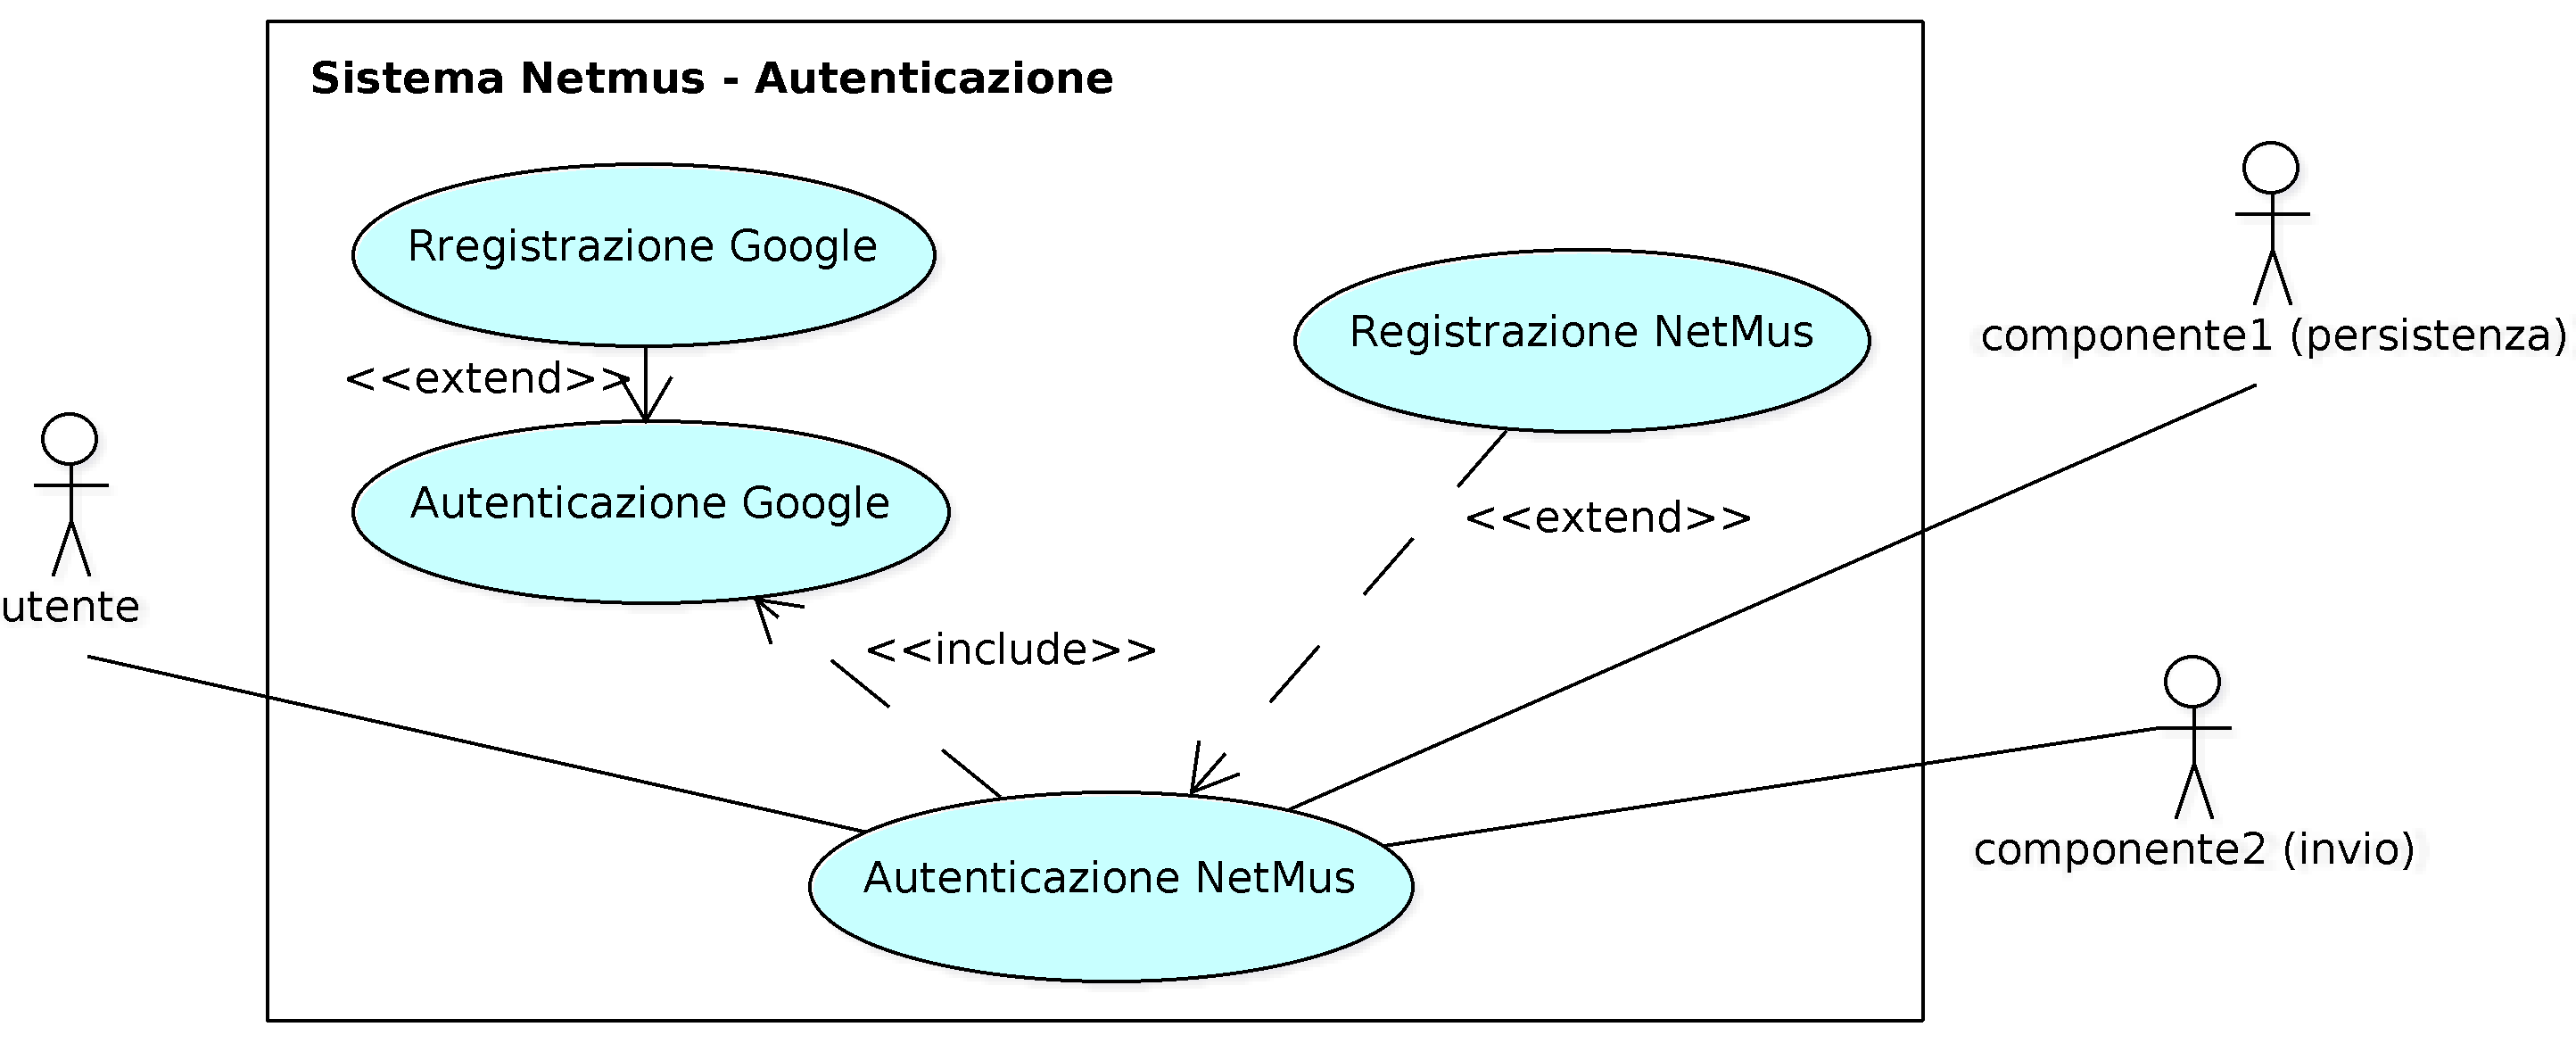
\includegraphics[width=14cm]{img/AR/UC1_1.png}
\caption{Diagramma dei casi d'uso che descrive le funzionalit\`a offerte
all'utente per quanto riguarda la gestione del proprio profilo personale.}
\end{figure}

\vspace*{0.5cm}
\bo{Use case UC1.1: Gestione del profilo personale} \\\\
\bo{Attori primari:} Utente. \\\\
\bo{Pre-condizioni:} Il portale \`e attivo ed ha in memoria, pronti all'utilizzo,
i dati relativi all'utente che si \`e autenticato.  \\\\ 
\bo{Post-condizioni:} L'utente ha effettuato tutte le operazioni desiderate con
successo. Il sistema ha salvato tutte le modifiche richieste. \\\\
\bo{Scenario principale:} 
\begin{enumerate}
  \item L'utente naviga all'interno della pagina di gestione del proprio profilo
  (UC1.1) in cui pu\`o accedere a tutte le informazioni personali salvate da
  NetMus che lo riguardano.
  \item L'utente fa alcune operazioni consentite come modificare alcuni
  dati (UC1.1.3), rendere visibile a tutti il proprio profilo e di conseguenza
  il proprio catalogo (UC1.1.2) oppure ha la possibilit\`a di cancellare la
  propria registrazione e rinunciare al servizio offerto da NetMus perdendo le
  informazioni raccolte fino a quel momento (UC1.1.1, UC1.1.4).
  \item Tutte le operazioni richieste dall'utente vengono eseguite in tempo
  utile dal server.
\end{enumerate}
\bo{Scenari secondari:}
\begin{itemize}
  \item La comunicazione tra utente e server fallisce per un problema di
  connessione.
  \begin {enumerate}
    \item Non c'\`e possibilit\`a di procedere fino a quando la connessione sar\`a
    ristabilita. I dati che erano stati aggiornati prima del verificarsi del
    problema sono gi\`a stati salvati.
  \end{enumerate}
\end{itemize}
\newpage

\section{UC1.3 - Gestione della libreria musicale}
\begin{figure}[h]
  \centering
  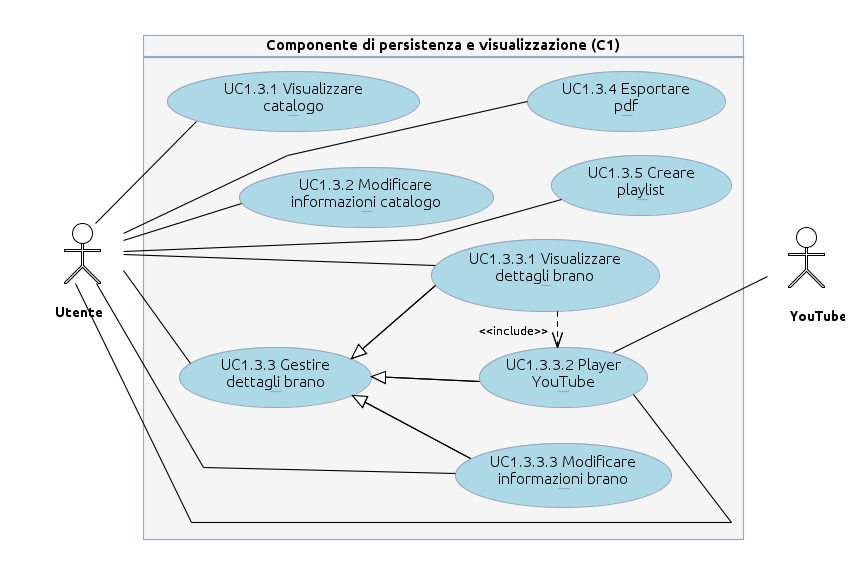
\includegraphics[width=18cm]{img/AR/UC1_3.png}
\caption{Diagramma dei casi d'uso che descrive come l'utente pu\`o gestire il
proprio catalogo di brani musicali.}
\end{figure}

\vspace*{0.5cm}
\bo{Use case UC1.3: Gestione della libreria musicale} \\\\
\bo{Attori primari:} Utente. \\\\
\bo{Attori secondari:} \underline{YouTube}. \\\\
\bo{Pre-condizioni:} Il portale \`e attivo ed ha in memoria, pronti all'utilizzo,
i dati relativi all'utente che si \`e autenticato.  \\\\ 
\bo{Post-condizioni:} L'utente \`e riuscito a vedere tutte le informazioni
salvate nella sua libreria musicale, sia quelle inviate dal suo computer sia
quelle aggiuntive recuperate dal database (UC1.3.1, UC1.3.3.1). L'utente ha
inoltre personalizzato il proprio catalogo a piacimento (UC1.3.2, UC1.3.3.3).
Il sistema ha salvato tutte le modifiche richieste e le sue funzionalit\`a sono
ancora tutte funzionanti e disponibili. \\\\
\bo{Scenario principale:} 
\begin{enumerate}
  \item L'utente visualizza la propria libreria di canzoni
  opportunamente raggruppate, la visualizzazione \`e simile a quella
  del software \underline{iTunes}.
  \item L'utente compie alcune tra le operazioni possibili sul proprio
  catalogo (UC1.3.2, UC1.3.4, UC1.3.5) oppure seleziona il brano che gli
  interessa e ne visualizza ed amministra i dettagli (UC1.3.3, UC1.3.3.1,
  UC1.3.3.2, UC1.3.3.3). Inoltre c'\`e anche il player YouTube (UC1.3.3.2) che
  gli permette di ascoltare la canzone in streaming.
  \item Il server o, nel caso venga chiesta la riproduzione del brano (UC1.3.3.2), il
  servizio esterno YouTube invia la pagina che l'utente ha richiesto e se
  necessario salva l'aggiornamento sui dati che ha fatto.
\end{enumerate}
\bo{Scenari secondari:}
\begin{itemize}
  \item La comunicazione tra utente e server fallisce per un problema di
  connessione.
  \begin {enumerate}
    \item Non c'\`e possibilit\`a di procedere fino a quando la connessione sar\`a
    ristabilita. I dati che erano stati aggiornati prima del verificarsi del
    problema sono gi\`a stati salvati.
  \end{enumerate}
  \item L'applicazione non ha trovato nessun corrispettivo del brano
  selezionato su YouTube.
  \begin {enumerate}
    \item Il player (UC1.3.3.2) non viene visualizzato ma tutte le altre
    funzionalit\`a rimangono invariate.
  \end{enumerate}
\end{itemize}
\newpage


\section{UC1.2 - Interazione con altri cataloghi}
\begin{figure}[h]
  \centering
  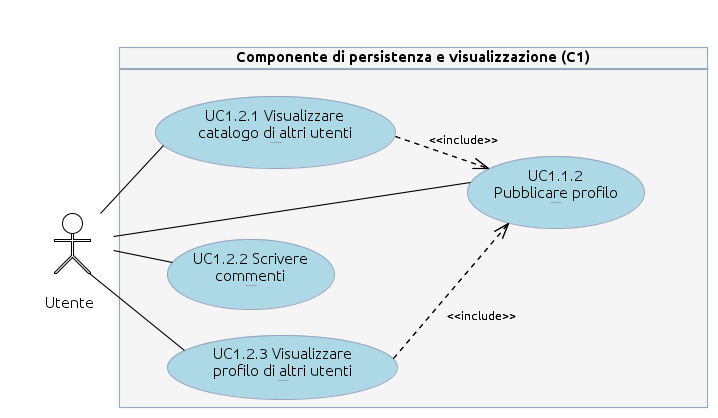
\includegraphics[width=15cm]{img/AR/UC1_2.png}
\caption{Diagramma dei casi d'uso che descrive le funzionalit\`a della componente
1 riguardanti l'interazione di un utente con tutti gli altri.}
\end{figure}

\vspace*{0.5cm}
\bo{Use case UC1.2: Interazione con altri cataloghi} \\\\
\bo{Attori primari:} Utente. \\\\
\bo{Pre-condizioni:} Il portale \`e attivo ed ha in memoria, pronti all'utilizzo,
i dati relativi all'utente che si \`e autenticato.  \\\\
\bo{Post-condizioni:} L'utente ha effettuato tutte le operazioni desiderate
con successo. Le funzionalit\`a del sistema sono ancora tutte funzionanti e
disponibili. \\\\
\bo{Scenario principale:} 
\begin{enumerate}
  \item L'utente rende pubblico e quindi visibile a tutti il proprio profilo
  (UC1.1.2).
  \item L'utente naviga all'interno del profilo o del catalogo musicale di un
  altro utente che ha pubblicato il proprio profilo (UC1.2.1, UC1.2.3).
  \item L'utente, se desidera, lascia alcuni commenti sul catalogo o profilo che
  sta visualizzando. (UC1.2.2).
  \item Tutti i dati richiesti dall'utente gli vengono forniti in tempo utile
  dal server.
\end{enumerate}
\bo{Scenari secondari:}
\begin{itemize}
  \item La comunicazione tra utente e server fallisce per un problema di
  connessione.
  \begin {enumerate}
    \item Non c'\`e possibilit\`a di procedere fino a quando la connessione sar\`a
    ristabilita. I dati che erano stati aggiornati prima del verificarsi del
    problema sono gi\`a stati salvati.
  \end{enumerate}
  \item L'utente cerca di accedere ad un altro catalogo (UC1.2.1, UC1.2.3) senza aver reso
  pubblico il proprio (UC1.2.2).
  \begin {enumerate}
    \item Viene chiesto all'utente se vuole pubblicare la propria libreria
    (UC1.2.2).
    \item In caso affermativo l'utente pu\`o procede a visualizzare altri
    cataloghi (UC1.2.1, UC1.2.3), altrimenti gli viene negato l'accesso e viene rimandato alla
    propria pagina (UC1.1).
  \end{enumerate}
\end{itemize}
\newpage

\section{UC2.2 - Inviare nuovi brani}
\begin{figure}[h]
  \centering
  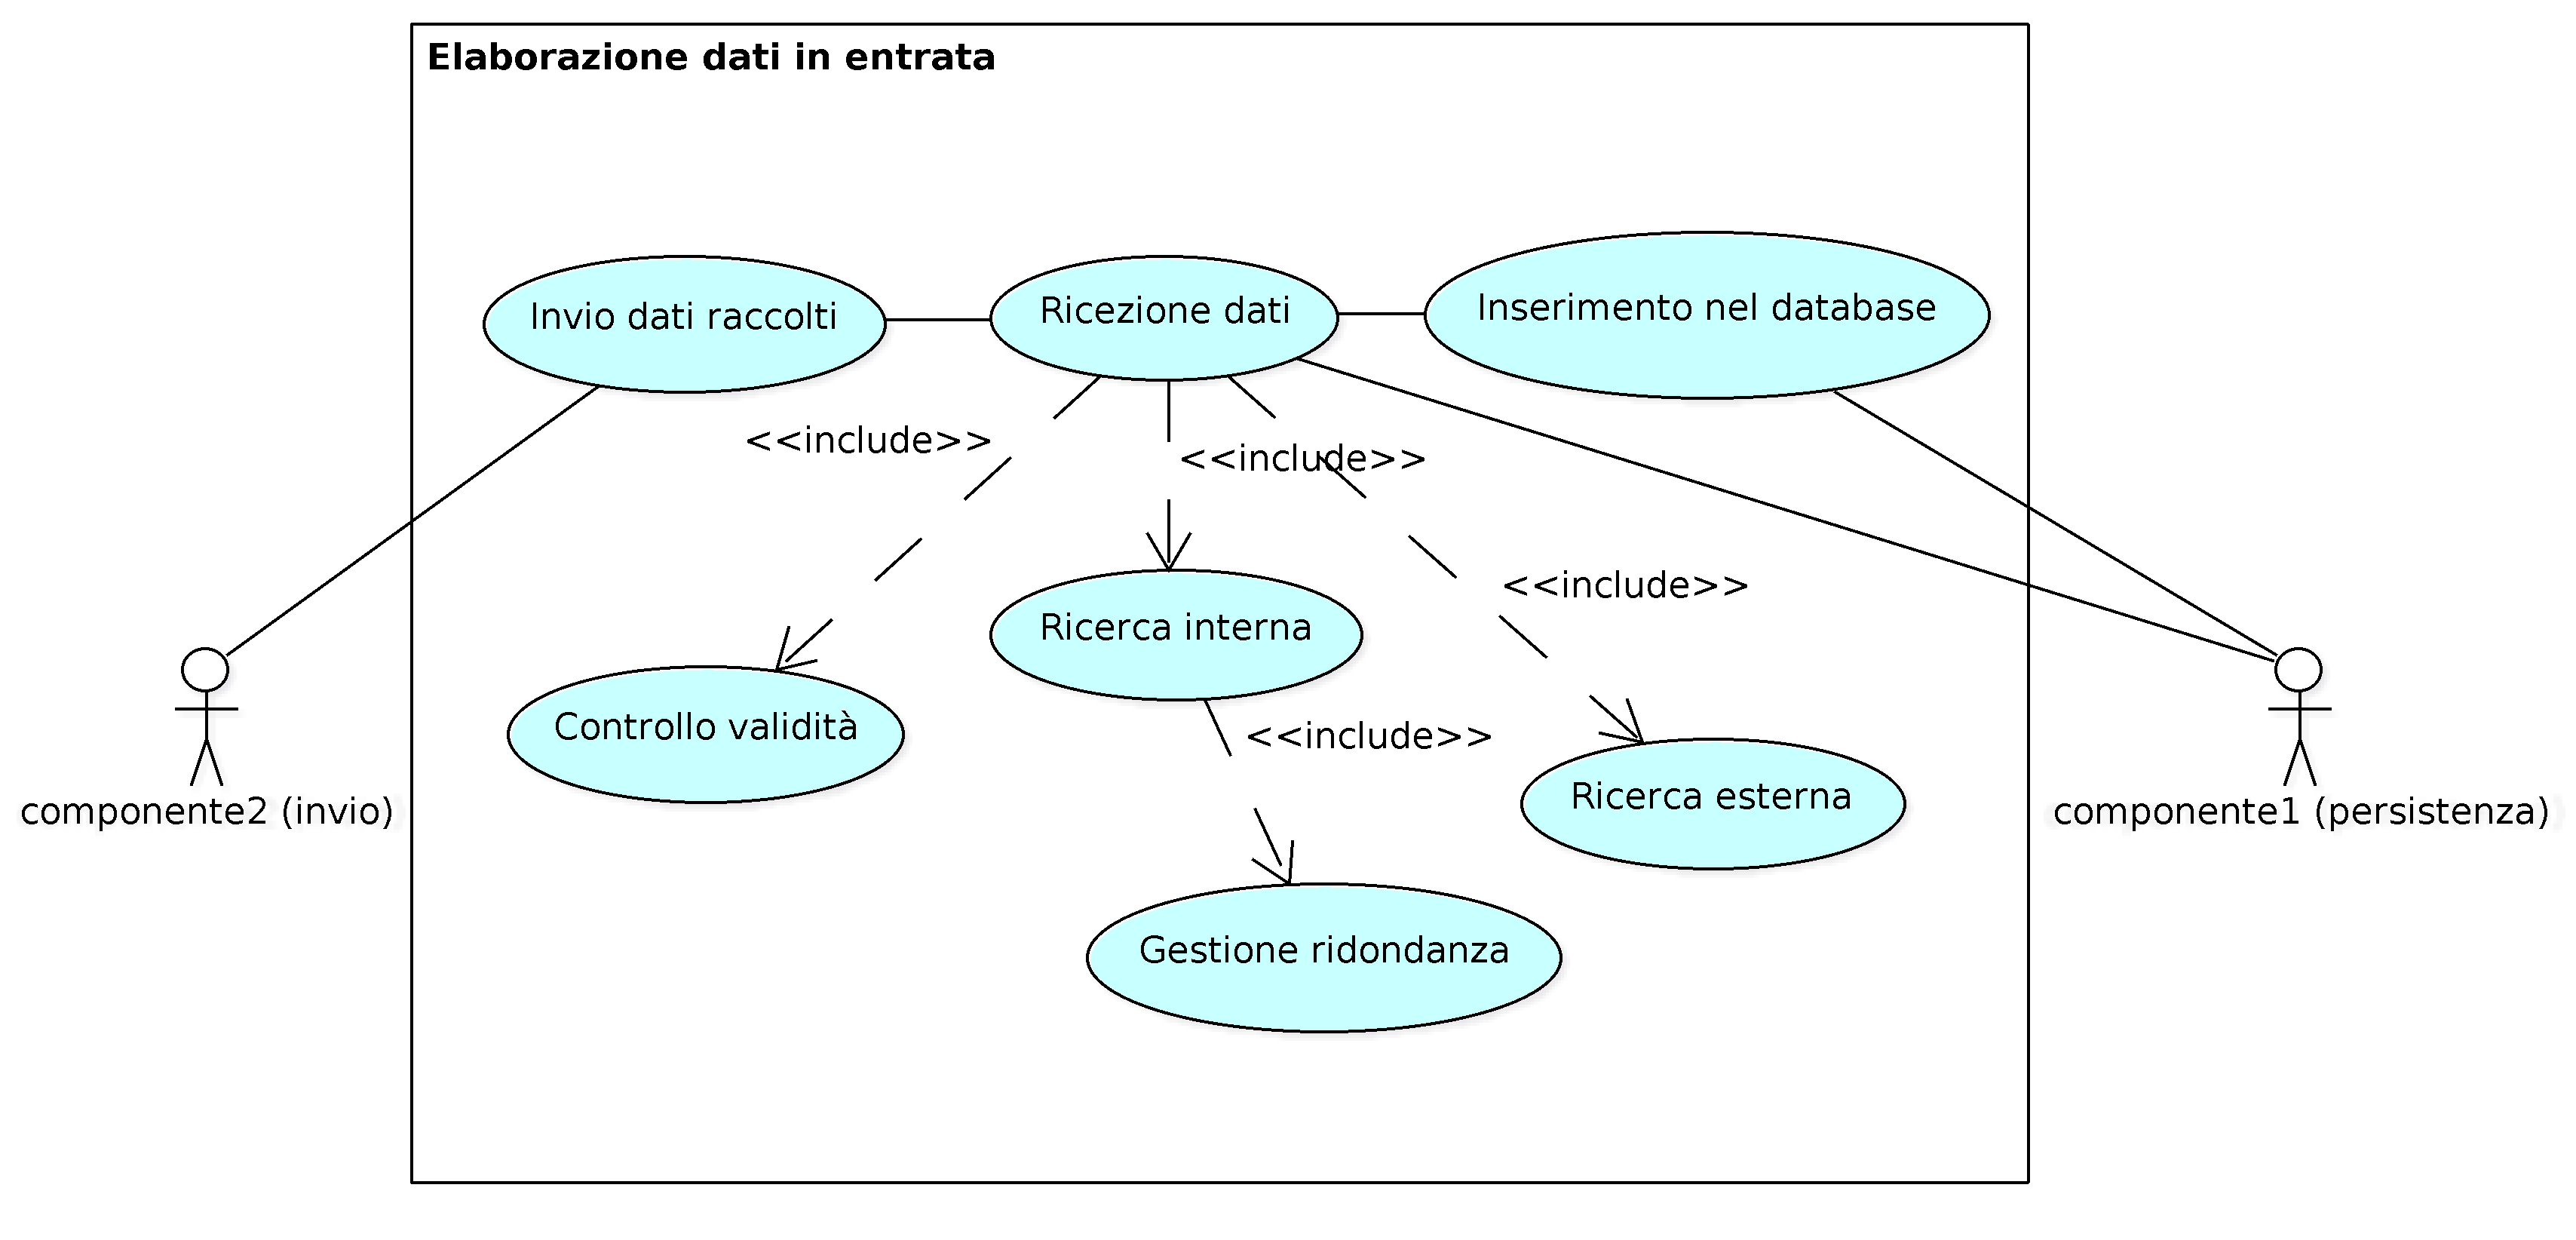
\includegraphics[width=10cm]{img/AR/UC2_2.png}
\caption{Diagramma dei casi d'uso che descrive le funzionalit\`a offerte
all'utente dalla componente 2 per inviare le nuove informazioni musicali al
database di NetMus.}
\end{figure}

\vspace*{0.5cm}
\bo{Use case UC2.2: Inviare nuovi brani}\\\\
\bo{Attori primari:} Utente. \\\\ 
\bo{Pre-condizioni:} La componente 2 del sistema NetMus \`e attiva poich\'e acceduta
dall'utente, quest'ultimo \`e autenticato. \\\\
\bo{Post-condizioni:} La componente 2 \`e ancora attiva e l'utente \`e pronto a
compiere qualsiasi altra operazione consentita dal sistema. Le nuove
informazioni reperite sono state tutte inviate al database di NetMus.\\\\
\bo{Scenario principale:}
\begin{enumerate}
  \item L'utente inserisce una nuova periferica USB (UC2.2.1), oppure avvia una
  scansione manuale (UC2.2.2).
  \item Tutti i dati raccolti riguardanti brani musicali vengono inviati a
  NetMus.
\end{enumerate}
\bo{Scenari secondari:}
\begin{itemize}
  \item La comunicazione fallisce per un problema di connessione.
  \begin {enumerate}
    \item Non c'\`e possibilit\`a di procedere con l'invio dei dati fino a
    quando la connessione sar\`a ristabilita.
  \end{enumerate}
\end{itemize}
\newpage


\chapter{Lista dei requisiti}
\thispagestyle{fancy}
Ad ogni requisito \`e stato assegnato un codice di identificazione per facilitarne
il tracciamento, per maggiori informazioni che riguardano la notazione
utilizzata per catalogare i requisiti si veda il documento
\emph{NormeDiProgetto-\versionenormeprogetto.pdf}.

\section{Componente di persistenza e visualizzazione (C1)}
\subsection{Requisiti funzionali}

\subsubsection*{WEB Application NetMus}
\bo{Id:} C1FN-1 \\
\bo{Tipo:} funzionale \\
\bo{Richiesta:} obbligatorio \\
\bo{Fonte:} capitolato\\
La Componente 1 del software NetMus deve permettere la gestione di un catalogo
multimediale virtuale ad ogni utente che ha effettuato la registrazione.
Deve essere accessibile all'utente come \underline{applicazione WEB}.

\subsubsection*{Grafica simile ad iTunes}
\bo{Id:} C1FN-1.1 \\
\bo{Tipo:} funzionale \\
\bo{Richiesta:} obbligatorio \\
\bo{Fonte:} capitolato \\
L'interfaccia grafica deve dare un'esperienza di visualizzazione simile alla
libreria musicale fornita dal software iTunes (\url{http://www.apple.com/it/itunes/}).

\subsubsection*{Elenco brani}
\bo{Id:} C1FN-1.1.1 \\
\bo{Tipo:} funzionale \\
\bo{Richiesta:} obbligatorio \\
\bo{Fonte:} capitolato \\
La parte principale della visualizzazione della libreria \`e costituita
dall'elenco dei brani dell'utente opportunamente raggruppati e catalogati.

\subsubsection*{Menu laterali}
\bo{Id:} C1FN-1.1.2 \\
\bo{Tipo:} funzionale \\
\bo{Richiesta:} obbligatorio \\
\bo{Fonte:} capitolato \\
Come avviene in iTunes la navigazione tra le varie pagine deve essere favorita
da un comodo men\`u laterale alla sinistra della finestra dei brani.

\subsubsection*{Informazioni dettagliate brano}
\bo{Id:} C1FN-1.1.3 \\
\bo{Tipo:} funzionale \\
\bo{Richiesta:} obbligatorio \\
\bo{Fonte:} capitolato \\
Per ognuno dei propri brani catalogati sar\`a possibile accedere alle informazioni
dettagliate in una nuova finestra, come ad esempio la copertina dell'album.

\subsubsection*{Player YouTube}
\bo{Id:} C1FD-1.1.4 \\
\bo{Tipo:} funzionale \\
\bo{Richiesta:} desiderabile \\
\bo{Fonte:} capitolato \\
Insieme alle informazioni di un brano dovrebbe comparire anche un player fornito
da YouTube con cui ascoltarlo.

\subsubsection*{Registrazione}
\bo{Id:} C1FN-1.2 \\
\bo{Tipo:} funzionale \\
\bo{Richiesta:} obbligatorio \\
\bo{Fonte:} capitolato \\
Un individuo pu\`o diventare utente di Netmus ed avere la possibilit\`a di gestire
il proprio catalogo multimediale solamente dopo aver effettuato la
registrazione, che prevede l'inserimento di un \underline{username} (unico), una
password, un indirizzo email (attraverso cui fare la conferma) e alcune
informazioni personali.

\subsubsection*{Pagina di login}
\bo{Id:} C1FN-1.2.1 \\
\bo{Tipo:} funzionale \\
\bo{Richiesta:} obbligatorio \\
\bo{Fonte:} verbale1 \\
L'applicazione avr\`a due sistemi di autenticazione: il proprio e quello di
Google.

\subsubsection*{Personalizzazione catalogo}
\bo{Id:} C1FN-1.3 \\
\bo{Tipo:} funzionale \\
\bo{Richiesta:} obbligatorio \\
\bo{Fonte:} interna \\
La gestione del catalogo prevede alcuni metodi di personalizzazione basilari che
permettono all'utente di visualizzare la propria libreria nel modo preferito,
senza modificare le informazioni a livello di database.

\subsubsection*{Cancellazione brano}
\bo{Id:} C1FN-1.3.1 \\
\bo{Tipo:} funzionale \\
\bo{Richiesta:} obbligatorio \\
\bo{Fonte:} verbale1 \\
Un utente potr\`a rimuovere dalla propria libreria qualche brano, per\`o i dati
rimarranno nel database.

\subsubsection*{Modifica informazioni brano}
\bo{Id:} C1FD-1.3.2 \\
\bo{Tipo:} funzionale \\
\bo{Richiesta:} desiderabile \\
\bo{Fonte:} interna \\
Tutte le informazioni di un brano potranno essere modificate dall'utente che le
ha caricate, il database non risentir\`a di questi cambiamenti e quindi anche
gli altri utenti non ne risentiranno in alcun modo.

\subsubsection*{Creazione playlist}
\bo{Id:} C1FO-1.3.3 \\
\bo{Tipo:} funzionale \\
\bo{Richiesta:} opzionale \\
\bo{Fonte:} interna \\
Viene data all'utente la possibilit\`a di creare delle liste lunghe a piacere
con i propri brani allo scopo di ordinare la propria libreria oppure di
ascoltarle in sequenza attraverso i player.

\subsubsection*{Ranking brani}
\bo{Id:} C1FO-1.3.4 \\
\bo{Tipo:} funzionale \\
\bo{Richiesta:} opzionale \\
\bo{Fonte:} interna \\
L'utente pu\`o assegnare un punteggio ad ogni brano in base al suo gradimento
personale e questo pu\`o tornare utile come criterio di ordinamento.

\subsubsection*{Gestione profilo personale}
\bo{Id:} C1FN-1.4 \\
\bo{Tipo:} funzionale \\
\bo{Richiesta:} obbligatorio \\
\bo{Fonte:} interna \\
In ogni momento l'utente di NetMus pu\`o modificare i suoi dati di registrazione,
eccetto l'username. Se desiderato il profilo pu\`o diventare pubblico ed essere
visibile agli altri utenti in modo da offrire la possibilit\`a di
confrontare il proprio catalogo musicale con quello degli altri.

\subsubsection*{Modifica informazioni personali}
\bo{Id:} C1FN-1.4.1 \\
\bo{Tipo:} funzionale \\
\bo{Richiesta:} obbligatorio \\
\bo{Fonte:} interna \\
Una volta effettuato il login sar\`a possibile accedere ad una pagina apposita per
aggiornare ed aggiungere informazioni al proprio profilo.

\subsubsection*{Cambio password}
\bo{Id:} C1FN-1.4.2 \\
\bo{Tipo:} funzionale \\
\bo{Richiesta:} obbligatorio \\
\bo{Fonte:} interna \\
Quando l'utente lo desidera pu\`o cambiare la password del proprio account.

\subsubsection*{Cancellazione account}
\bo{Id:} C1FN-1.4.3 \\
\bo{Tipo:} funzionale \\
\bo{Richiesta:} obbligatorio \\
\bo{Fonte:} interna \\
Deve essere possibile per ogni utente chiudere il proprio profilo in maniera
permanente eliminando dal database ogni sua informazione.

\subsubsection*{Pubblicazione profilo}
\bo{Id:} C1FD-1.4.4 \\
\bo{Tipo:} funzionale \\
\bo{Richiesta:} desiderabile \\
\bo{Fonte:} interna \\
Per interagire con gli altri sar\`a necessario pubblicare il proprio profilo e
di conseguenza la propria libreria di canzoni rendendo visibile a tutti ci\`o che
contengono.

\subsubsection*{Riproduzione tracce in streaming}
\bo{Id:} C1FD-1.5 \\
\bo{Tipo:} funzionale \\
\bo{Richiesta:} desiderabile \\
\bo{Fonte:} capitolato \\
NetMus prevede un sistema di riproduzione delle canzoni salvate nel database.
Non contenendo alcun file multimediale l'ascolto sar\`a reso possibile dalla
riproduzione in streaming fornita da YouTube. La ricerca dei brani
corrispondenti alle informazioni nel database sar\`a a totale carico
dell'applicazione NetMus.

\subsubsection*{Interazione con altri utenti}
\bo{Id:} C1FD-1.7 \\
\bo{Tipo:} funzionale \\
\bo{Richiesta:} desiderabile \\
\bo{Fonte:} interna \\
La comunicazione con altri utenti sar\`a favorita da alcune semplici funzionalit\`a
che rendono la propria libreria oggetto di confronto dando pi\`u spazio
allo scambio di idee e conoscenze tra gli utilizzatori di NetMus.

\subsubsection*{Visualizzazione altri profili}
\bo{Id:} C1FD-1.7.1 \\
\bo{Tipo:} funzionale \\
\bo{Richiesta:} desiderabile \\
\bo{Fonte:} interna \\
Sar\`a possibile visualizzare l'intera libreria musicale e le altre informazioni
di tutti gli utenti che hanno permesso la condivisione del proprio profilo.

\subsubsection*{Lasciare commenti}
\bo{Id:} C1FO-1.7.2 \\
\bo{Tipo:} funzionale \\
\bo{Richiesta:} opzionale \\
\bo{Fonte:} interna \\
Uno strumento semplice ma molto coinvolgente sar\`a la possibilit\`a di scrivere
commenti alle informazioni condivise da altri utenti come brani, autori e
playlist.

\subsubsection*{Elaborazione dati utente}
\bo{Id:} C1FD-1.8 \\
\bo{Tipo:} funzionale \\
\bo{Richiesta:} desiderabile \\
\bo{Fonte:} interna \\
Il sistema NetMus si occuper\`a anche di elaborare in modo intelligente i dati
raccolti dai vari utenti permettendo di avere nel proprio profilo dei dati
riassuntivi riguardanti la propria libreria ma anche di avere delle informazioni
di confronto con le librerie degli altri utenti.

\subsubsection*{Esportazione pdf}
\bo{Id:} C1FO-1.8.1 \\
\bo{Tipo:} funzionale \\
\bo{Richiesta:} opzionale \\
\bo{Fonte:} interna \\
Sar\`a possibile esportare il proprio catalogo opportunamente indicizzato e con
informazioni aggiuntive procurate da NetMus in formato \underline{pdf}
predisposto per la stampa.

\subsubsection*{Ricezione ed elaborazione brani}
\bo{Id:} C1FN-1.9 \\
\bo{Tipo:} funzionale \\
\bo{Richiesta:} obbligatorio \\
\bo{Fonte:} capitolato \\
Netmus deve occuparsi della ricezione dei dati in arrivo da tutte le componenti
di invio che si connettono ad esso, dovr\`a quindi gestire queste connessioni in
modo concorrente nel miglior modo possibile. Inoltre per tutte le informazioni
ricevute con successo si occuper\`a di verificarne la validit\`a e di arricchirne i
contenuti ove possibile.

\subsubsection*{Controllo validit\`a dati}
\bo{Id:} C1FN-1.9.1 \\
\bo{Tipo:} funzionale \\
\bo{Richiesta:} obbligatorio \\
\bo{Fonte:} capitolato \\
Tutte le informazioni inviate da C2 saranno controllate in maniera
rapida ma che garantisca che non vi siano dati maligni per NetMus o che non
riguardino brani musicali.

\subsubsection*{Completamento informazioni da database interno}
\bo{Id:} C1FN-1.9.2 \\
\bo{Tipo:} funzionale \\
\bo{Richiesta:} obbligatorio \\
\bo{Fonte:} interna \\
Sar\`a sfruttato il database interno per completare ed aggiungere informazioni
mancanti ai brani in entrata. Questo sar\`a fatto basandosi su opportuni algoritmi
di ricerca che garantiscano una buona probabilit\`a che i dati suggeriti per
l'aggiornamento siano quelli corretti.

\subsubsection*{Inserimento nel database}
\bo{Id:} C1FN-1.9.5 \\
\bo{Tipo:} funzionale \\
\bo{Richiesta:} obbligatorio \\
\bo{Fonte:} capitolato \\
Una volta controllate ed aggiornate le informazioni ricevute verranno salvate
nel database entrando a far parte a tutti gli effetti della libreria musicale
dell'utente da cui sono state ricevute.

\subsubsection*{Completamento informazioni da servizio esterno}
\bo{Id:} C1FO-1.9.3 \\
\bo{Tipo:} funzionale \\
\bo{Richiesta:} opzionale \\
\bo{Fonte:} capitolato \\
Per reperire informazioni sicure che possano servire per correggere eventuali
dati mancanti riguardo i brani inviati a NetMus, se il database interno non le
possiede, si sfrutter\`a uno o pi\`u servizi gratuiti esterni.

\subsubsection*{Invio nuove informazioni a C2}
\bo{Id:} C1FD-1.10 \\
\bo{Tipo:} funzionale \\
\bo{Richiesta:} desiderabile \\
\bo{Fonte:} verbale1 \\
Se consultando il database interno o esterno saranno trovate informazioni
aggiuntive ai dati inviati da qualche utente e questo lo desidera, sar\`a
possibile inviarle a C2 per andare ad aggiornare i file multimediali
dell'utente.

\subsubsection*{Gestione database}
\bo{Id:} C1FN-1.13 \\
\bo{Tipo:} funzionale \\
\bo{Richiesta:} obbligatorio \\
\bo{Fonte:} capitolato \\
Il fulcro della persistenza del sistema NetMus sar\`a un database nel quale
verranno salvati tutti i dati gestiti. In particolare il database sar\`a Google
DataStore, fornito da Google AppEngine, che trae grandissimi benefici
dal cloud computing.

\subsection{Requisiti di qualit\`a}

\subsubsection*{Ottimizzazione della ricerca su YoutTube}
\bo{Id:} C1QD-1.5.1 \\
\bo{Tipo:} qualit\`a \\
\bo{Richiesta:} desiderabile \\
\bo{Fonte:} interna \\
YouTube \`e uno strumento estremamente utile perch\'e garantisce una vasta gamma
di dati sulla quale si possono fare ricerche e proprio per questo sar\`a
importante che NetMus implementi degli algoritmi opportuni per eseguire ricerche
in modo molto efficiente.

\subsubsection*{Identificazione dati ridondanti}
\bo{Id:} C1QN-1.9.4 \\
\bo{Tipo:} qualit\`a \\
\bo{Richiesta:} obbligatorio \\
\bo{Fonte:} interna \\
NetMus sar\`a in grado di associare le informazioni simili e
riguardanti lo stesso brano in modo da inserirle una sola vola all'interno del
database. Questo verr\`a fatto solo se si ha la sicurezza che si tratti dello
stesso brano, altrimenti verranno mantenute le diverse versioni fino a quando si
avranno informazioni sufficienti per saperlo.

\subsubsection*{Gestione concorrenza}
\bo{Id:} C1QN-1.9.6 \\
\bo{Tipo:} qualit\`a \\
\bo{Richiesta:} obbligatorio \\
\bo{Fonte:} interna \\
La componente di persistenza sar\`a in grado di gestire la concorrenza tra le
richieste di invio dati simultanee da vari clients in modo da garantire una
corretta ricezione di tutte le informazioni.

\subsubsection*{Scalabilit\`a}
\bo{Id:} C1QN-1.6 \\
\bo{Tipo:} qualit\`a \\
\bo{Richiesta:} obbligatorio \\
\bo{Fonte:} capitolato \\
NetMus garantir\`a la possibilit\`a di crescere di dimensione, in tutti i vari
aspetti, senza dover effettuare alcun ritocco o modifica all'architettura del
sistema.

\subsubsection*{Scalabilit\`a interfaccia grafica}
\bo{Id:} C1QN-1.6.1 \\
\bo{Tipo:} qualit\`a \\
\bo{Richiesta:} obbligatorio \\
\bo{Fonte:} capitolato \\
La libreria personale dell'utente sar\`a potenzialmente infinita, di conseguenza
le pagine che ne permetteranno la visualizzazione saranno in grado di adattarsi
senza imporre vincoli di alcun tipo.

\subsubsection*{Scalabilit\`a massa di utenza}
\bo{Id:} C1QN-1.6.2 \\
\bo{Tipo:} qualit\`a \\
\bo{Richiesta:} obbligatorio \\
\bo{Fonte:} capitolato \\
Poich\'e il bacino d'utenza potenziale \`e estremamente elevato NetMus sar\`a molto
efficiente per quanto riguarda gli accessi simultanei di molti utenti
all'applicazione web e al database.

\subsubsection*{Utilizzo}
\bo{Id:} C1QN-2 \\
\bo{Tipo:} qualit\`a \\
\bo{Richiesta:} obbligatorio \\
\bo{Fonte:} interna \\
Un occhio di riguardo sar\`a dato alla semplicit\`a di utilizzo e alla
possibilit\`a per tutti i potenziali utenti di imparare ad utilizzare NetMus. L'utente
deve poter essere subito in grado di visualizzare e gestire il proprio catalogo
musicale dopo essersi registrato e aver messo in funzione la C2.

\subsubsection*{Accessibilit\`a}
\bo{Id:} C1QO-2.1 \\
\bo{Tipo:} qualit\`a \\
\bo{Richiesta:} opzionale \\
\bo{Fonte:} interna \\
Il software Web presenter\`a alcune caratteristiche per favorire l'accesso a
qualsiasi tipologia di utenza come ad esempio il \underline{codice sorgente}
validato secondo parametri \underline{W3C}.

\subsubsection*{Portabilit\`a}
\bo{Id:} C1QN-2.3 \\
\bo{Tipo:} qualit\`a \\
\bo{Richiesta:} obbligatorio \\
\bo{Fonte:} interna \\
Deve essere compatibile col maggior numero di configurazioni software e
hardware.

\subsubsection*{Supporto multi-lingua}
\bo{Id:} C1QD-2.4 \\
\bo{Tipo:} qualit\`a \\
\bo{Richiesta:} desiderabile \\
\bo{Fonte:} capitolato \\
Saranno accessibili due versioni dell'applicazione, una in italiano ed una in
lingua inglese, con gli stessi contenuti e sar\`a possibile spostarsi da una
all'altra in qualsiasi momento.

\subsubsection*{Manutenibilit\`a}
\bo{Id:} C1QN-2.6 \\
\bo{Tipo:} qualit\`a \\
\bo{Richiesta:} obbligatorio \\
\bo{Fonte:} interna \\
Saranno seguiti dei criteri di scrittura del codice e stesura dei documenti che
favoriranno il pi\`u possibile il processo di manutenzione.

\subsubsection*{Gestione errori}
\bo{Id:} C1QN-2.7 \\
\bo{Tipo:} qualit\`a \\
\bo{Richiesta:} obbligatorio \\
\bo{Fonte:} interna \\
Il sistema sar\`a robusto relativamente agli errori causati all'utilizzo della
rete internet, notoriamente inaffidabile.

\subsubsection*{Manuale utente}
\bo{Id:} C1QN-3.1 \\
\bo{Tipo:} qualit\`a \\
\bo{Richiesta:} obbligatorio \\
\bo{Fonte:} capitolato \\
Sar\`a redatto un manuale utente che conterr\`a tutte e sole le informazioni
necessarie all'utilizzo di NetMus in modo da essere facilmente comprensibile da
tutta l'enorme fascia di utenza a cui si rivolge.

\subsubsection*{Manuale utente inglese}
\bo{Id:} C1QD-3.1.1 \\
\bo{Tipo:} qualit\`a \\
\bo{Richiesta:} desiderabile \\
\bo{Fonte:} capitolato \\
Sar\`a fornita anche una traduzione del manuale utente in lingua inglese.


\subsection{Requisiti di vincolo}

\subsubsection{Interfacciamento con gli ambienti di installazione e d'uso }

\subsubsection*{Tecnologie GAE e GWT}
\bo{Id:} C1VN-1.12 \\
\bo{Tipo:} vincolo \\
\bo{Richiesta:} obbligatorio \\
\bo{Fonte:} capitolato \\
Per lo sviluppo dell'applicazione Web NetMus sar\`a utilizzata la piattaforma
Google App Engine (GAE) in concomitanza con l'insieme di strumenti forniti da Google Web Toolkit (GWT). Entrambi sono gratuiti.

\subsubsection*{Google DataStore}
\bo{Id:} C1VN-1.13.1 \\
\bo{Tipo:} vincolo \\
\bo{Richiesta:} obbligatorio \\
\bo{Fonte:} capitolato \\
Il database verr\`a sviluppato utilizzando \underline{Google DataStore}.

\subsubsection*{Cloud computing}
\bo{Id:} C1VN-1.11 \\
\bo{Tipo:} vincolo \\
\bo{Richiesta:} obbligatorio \\
\bo{Fonte:} capitolato \\
Sar\`a utilizzato il supporto al cloud computing fornito da Google AppEngine,
anche per quanto riguarda il database grazie a Google DataStore.

\subsubsection{Norme vigenti nel dominio applicativo}

\subsubsection*{Quote YouTube}
\bo{Id:} C1VD-1.5.2 \\
\bo{Tipo:} vincolo \\
\bo{Richiesta:} desiderabile \\
\bo{Fonte:} interna \\
NetMus rispetter\`a le quote di traffico imposte da YouTube per quanto riguarda
il traffico in entrata ed in uscita dai loro server.

\subsubsection*{YouTube Terms of Service}
\bo{Id:} C1VD-1.5.3 \\
\bo{Tipo:} vincolo \\
\bo{Richiesta:} desiderabile \\
\bo{Fonte:} interna \\
NetMus rispetter\`a le regole stabilite da YouTube per quanto riguarda i
propri contenuti \\(\url{http://www.YouTube.com/t/terms}) e per quanto
riguarda l'utilizzo delle YouTube API\\
(\url{http://code.google.com/apis/YouTube/terms.html}).

\subsubsection*{Open source}
\bo{Id:} C1VN-2.2 \\
\bo{Tipo:} vincolo \\
\bo{Richiesta:} obbligatorio \\
\bo{Fonte:} capitolato \\
La licenza d'uso dell'applicazione sar\`a di tipo \underline{Open source}.

\subsubsection{Caratteristiche dell'utente}

\subsubsection*{Semplicit\`a di utilizzo}
\bo{Id:} C1VN-2.5 \\
\bo{Tipo:} vincolo \\
\bo{Richiesta:} obbligatorio \\
\bo{Fonte:} interna \\
Tutte le componenti dell'applicazione Web NetMus saranno mirate alla semplicit\`a
di utilizzo da parte dell'utente. A partire dall'interfaccia grafica sar\`a tutto
molto intuitivo.


\subsection{Gerarchia dei requisiti}

\begin{table}[!h]
\centering
\begin{footnotesize}
\begin{tabular}{|l|l|}

\rowcolor{Orange}
\bo{Web Application Netmus} \\
\hline
\cellcolor{orange}
Grafica simile ad iTunes & Elenco brani raggruppati opportunamente \\
& Menu laterali \\   
& Visualizzazione informazioni dettagliate di un brano \\         
& Visualizza player YouTube \\         
\hline
\cellcolor{orange}
Creazione profilo utente tramite registrazione & Pagina di login dipendente da Google login \\ 
\hline
\cellcolor{orange}
Personalizzazione del proprio catalogo & Cancellazione brano \\
& Modifica informazioni brano \\       
& Creazione playlist \\
& Ranking brani \\   
\hline
\cellcolor{orange}
Gestione profilo personale & Modifica informazioni personali \\         
& Cambio password \\
& Cancellazione del proprio account \\       
& Pubblicazione profilo \\
\hline
\cellcolor{orange}
Riproduzione tracce in streaming & Ottimizzazione della ricerca su YouTube \\       
& Quote YouTube \\
& YouTube Terms of Service \\       
\hline
\cellcolor{orange}
Scalabilit\`a & Scalabilit\`a di interfaccia grafica \\       
& Scalabilit\`a di massa d'utenza \\   
\hline
\cellcolor{orange}
Interazione con altri utenti & Visualizzazione di altri profili \\        
& Lasciare commenti su altri profili \\         
\hline
\cellcolor{orange}
Elaborazione dati utente & Esportazione pdf \\
\hline
\cellcolor{orange}
Ricezione ed elaborazione brani & Controllo di validit\`a dati \\   
& Controllo informazioni da database interno \\       
& Identificazione di dati ridondanti \\
& Inserimento nel database \\
& Gestione concorrenza \\
& Completamento informazioni da servizio esterno \\         
\hline
\cellcolor{orange}
Invio nuove informazioni a Componente 2& \\       
\hline
\cellcolor{orange}
Deve utilizzare il cloud computing& \\
\hline
\cellcolor{orange}
Deve utilizzare tecnologie GAE e GWT& \\
\hline
\cellcolor{orange}
Gestione database & Deve utilizzare Google Datastore \\        
\hline
\end{tabular}
\\\vspace{1cm}
\begin{tabular}{|l|}
\hline
\rowcolor{Orange}
\bo{Utilizzo} \\
\hline
\rowcolor{orange}
 Accessibilit\`a \\
 \rowcolor{orange}                  
 Open source \\  
 \rowcolor{orange}         
 Portabilit\`a \\
 \rowcolor{orange}               
 Sviluppo multi-lingua \\
 \rowcolor{orange}                  
 Semplicit\`a di utilizzo \\
 \rowcolor{orange}               
 Manutenibilit\`a \\
 \rowcolor{orange}         
 Gestione errori \\             
\hline
\end{tabular}
\hspace{3cm}
\begin{tabular}{|l|}
\hline
\rowcolor{Orange}
\bo{Documenti} \\           
\hline
\rowcolor{orange}
 Manuale utente \\                 
\hline
\rowcolor{orange}
 Manuale utente inglese \\                  
\hline
\end{tabular}
\end{footnotesize}
\caption{Gerarchia dei requisiti (C1)}
\end{table}

\begin{sidewaystable}[]
\centering
\begin{footnotesize}
\begin{tabular}{|l|l|l|}
\rowcolor{Orange}
\bo{Requisiti Funzionali}\\
\hline
\rowcolor{orange}                         
\sca{Necessari} & \sca{Desiderabili} & \sca{Opzionali} \\         
C1FN-1 Web Application Netmus & C1FD-1.1.4 Visualizza player YouTube &
C1FO-1.2.1 Pagina login indipendente \\
C1FN-1.1 Grafica simile ad iTunes & C1FD-1.3 Personalizzazione del catalogo & C1FO-1.3.3 Creazione playlist \\
 C1FN-1.1.1 Brani elencati opportunamente & C1FD-1.3.1 Cancellazione brano & C1FO-1.3.4 Ranking brani \\ 
C1FN-1.1.2 Menu laterali & C1FD-1.3.2 Modifica informazioni brano & C1FO-1.7.2
Lasciare commenti su  \\ C1FN-1.1.3 Visualiz. info dettagliate dei brani & C1FD-1.4.4 Pubblicazione
profilo & C1FO-1.8.1 Esportazione PDF \\ C1FN-1.4 Gestione profilo personale &
C1FD-1.5 Riproduzione tracce in streaming & C1FO-1.9.3 Completamento info da  \\
C1FN-1.4.1 Modifica informazioni personali & C1FD-1.7 Interazione con altri utenti & \\       
C1FN-1.4.3 Cancellazione del proprio account & C1FD-1.7.1 Visualizzazione altri profili & \\                    
C1FN-1.9 Ricezione ed elaborazione dei brani & C1FD-1.8 Elaborazione dati utente &   \\             
C1FN-1.9.1 Controllo di validit\`a dei dati & C1FD-1.10 Invio nuove informazioni a C2 & \\                
C1FN-1.9.2 Completamento info da database interno & & \\                                 
C1FN-1.9.4 Identificazione dati ridondanti & & \\                         
C1FN-1.9.5 Inserimento nel Database & & \\                             
C1FN-1.13 Gestione Database &  & \\                   
\hline
\end{tabular}
\caption{Requisiti funzionali (C1)}

\begin{tabular}{|l|l|l|}
\cline{1-1}
\rowcolor{Orange}
\bo{Requisiti Di Qualit\`a} \\
\hline
\rowcolor{orange}                         
\sca{Necessari} & \sca{Desiderabili} & \sca{Opzionali} \\
C1QN-1.6 Scalabilit\`a & C1QN-1.5.1 Ottimizzazione della ricerca su YouTube & C1QO-2.1 Accessibilit\`a   \\ 
C1QN-1.6.1 Scalabilit\`a interfaccia grafica & C1QN-2.4 Supporto multilingua & \\                
C1QN-1.6.2 Scalabilit\`a massa di utenza  &  & \\                         
C1QN-1.9.6 Gestione concorrenza &  & \\                          
C1QN-2.3 Portabilit\`a &  & \\              
C1QN-2.7 Gestione errori &  &   \\       
C1QN-3.1 Manuale utente &  & \\                            
\hline
\end{tabular}
\caption{Requisiti di qualit\`a (C1)}
\end{footnotesize}
\end{sidewaystable}

% requisiti di vincolo

\begin{table}
\centering
\begin{footnotesize}
\begin{tabular}{|l|l|l|}
\cline{1-1}
\rowcolor{Orange}
\bo{Requisiti Di Vincolo}   \\
\hline
\rowcolor{orange}                         
\sca{Necessari} & \sca{Desiderabili} \\   
C1VN-1.12 Deve utilizzare tecnologie GAE e GWT & C1VD-1.5.2 Quote YouTube   \\ 
C1VN-1.13.1 Deve utilizzare Google Data Store & C1VD-1.5.3 YouTube Terms of
Services \\
C1VN-1.11 Deve utilizzare il cloud computing & \\  
C1VN-2.2 Open source & \\
C1VN-2.5 Semplicit\`a di utilizzo & \\
\hline
\end{tabular}
\caption{Requisiti di vincolo (C1)}
\end{footnotesize}
\end{table}

\newpage

%---------------

\section{Componente di recupero delle informazioni (C2)}

\subsection{Requisiti funzionali}
\subsubsection*{Recupero delle informazioni}
\bo{Id:} C2FN-1 \\
\bo{Tipo:} funzionale \\
\bo{Richiesta:} obbligatorio \\
\bo{Fonte:} capitolato \\
La Componente 2 deve recuperare le informazioni dei brani musicali dell'utente
per permettere alla Componente 1 di creare la libreria musicale virtuale.

\subsubsection*{Recupero automatico}
\bo{Id:} C2FN-1.1 \\
\bo{Tipo:} funzionale \\
\bo{Richiesta:} obbligatorio \\
\bo{Fonte:} capitolato \\
La Componente 2 deve recuperare le informazioni dei brani musicali
automaticamente all'inserimento di un nuovo dispositivo.

\subsubsection*{Recupero manuale}
\bo{Id:} C2FN-1.2 \\
\bo{Tipo:} funzionale \\
\bo{Richiesta:} obbligatorio \\
\bo{Fonte:} interna \\
Sotto comando dell'utente (alla pressione di un bottone) vengono recuperate le
informazioni di tutti i brani musicali nuovi rilevabili.

\subsubsection*{Informazioni senza connessione}
\bo{Id:} C2FO-1.3 \\
\bo{Tipo:} funzionale \\
\bo{Richiesta:} opzionale \\
\bo{Fonte:} verbale1 \\
Il recupero delle informazioni va effettuato anche con connessione non
disponibile, salvandolo temporaneamente in locale. Appena possibile queste
informazioni verranno trasmesse alla Componente 1.

\subsubsection*{Informazioni dall'hard disk}
\bo{Id:} C2FD-1.4 \\
\bo{Tipo:} funzionale \\
\bo{Richiesta:} desiderabile \\
\bo{Fonte:} interna \\
Vengono osservate per la ricerca di brani musicali anche le directory sull'hard
disk indicate dall'utente.

\subsubsection*{File ignorati}
\bo{Id:} C2FN-1.5 \\
\bo{Tipo:} funzionale \\
\bo{Richiesta:} obbligatorio \\
\bo{Fonte:} verbale1 \\
Tutti i brani musicali senza informazioni rintracciabili, cio\`e senza meta-tag e
senza nome del brano nel nome del file, verranno ignorati perch\'e inutili ai fini
del progetto.

\subsubsection*{Indicazioni file ignorati}
\bo{Id:} C2FO-1.6 \\
\bo{Tipo:} funzionale \\
\bo{Richiesta:} opzionale \\
\bo{Fonte:} interna \\
Vengono indicati all'utente i file musicali non tracciati perch\'e senza
sufficienti informazioni.

\subsubsection*{Aggiornamento e completamento informazioni}
\bo{Id:} C2FD-2 \\
\bo{Tipo:} funzionale \\
\bo{Richiesta:} desiderabile \\
\bo{Fonte:} verbale1 \\
Sotto richiesta esplicita dell'utente (alla pressione di un bottone) vengono
aggiornate e completate, ove possibile, le informazioni sui file dell'utente,
prelevate dalla componente 1.

\subsubsection*{Comunicazione con C1}
\bo{Id:} C2FN-3 \\
\bo{Tipo:} funzionale \\
\bo{Richiesta:} obbligatorio \\
\bo{Fonte:} capitolato \\
La Componente 2 comunica attraverso la connessione internet con la Componente 1.

\subsubsection*{Invio delle informazioni}
\bo{Id:} C2FN-3.1 \\
\bo{Tipo:} funzionale \\
\bo{Richiesta:} obbligatorio \\
\bo{Fonte:} capitolato \\
Invio delle informazioni sui brani raccolte alla Componente 1 per permettere la
generazione e/o l'aggiornamento della raccolta virtuale.

\subsection{Requisiti di qualit\`a}
\subsubsection*{Ottimizzazione memoria cache}
\bo{Id:} C2QD-1.7 \\
\bo{Tipo:} qualit\`a \\
\bo{Richiesta:} desiderabile \\
\bo{Fonte:} verbale1 \\
In caso di connessione non disponibile, deve utilizzare meno spazio possibile
per memorizzare temporaneamente i dati dei nuovi brani, per poi eliminare i file
temporanei appena questi dati non sono pi\`u necessari.

\subsubsection*{Utilizzo della connessione}
\bo{Id:} C2QN-3.2 \\
\bo{Tipo:} qualit\`a \\
\bo{Richiesta:} obbligatorio \\
\bo{Fonte:} verbale1 \\
Vanno evitate le comunicazioni inutili con la Componente 1, limitandosi allo
stretto necessario.

\subsubsection*{Utilizzo}
\bo{Id:} C2QN-4\\
\bo{Tipo:} qualit\`a \\
\bo{Richiesta:} obbligatorio \\
\bo{Fonte:} interna \\
La componente dev'essere alla portata di qualsiasi tipologia di utente.

\subsubsection*{Portabilit\`a}
\bo{Id:} C2QD-4.1\\
\bo{Tipo:} qualit\`a \\
\bo{Richiesta:} desiderabile \\
\bo{Fonte:} verbale1 \\
Deve essere compatibile col maggior numero di configurazioni software e
hardware.

\subsubsection*{Semplicit\`a di utilizzo}
\bo{Id:} C2QD-4.2\\
\bo{Tipo:} qualit\`a \\
\bo{Richiesta:} obbligatorio \\
\bo{Fonte:} interna \\
Deve essere semplice ed intuitiva da utilizzare.

\subsubsection*{Supporto multi-lingua}
\bo{Id:} C2QD-4.3\\
\bo{Tipo:} qualit\`a \\
\bo{Richiesta:} desiderabile \\
\bo{Fonte:} capitolato \\
La componente potr\`a essere configurata per utilizzare una specifica lingua tra
quelle disponibili (italiano ed inglese).

\subsubsection*{Manutenibilit\`a}
\bo{Id:} C2QN-4.4\\
\bo{Tipo:} qualit\`a \\
\bo{Richiesta:} obbligatorio \\
\bo{Fonte:} interna \\
Saranno seguiti dei criteri di scrittura del codice e stesura dei documenti che
favoriranno il pi\`u possibile il processo di manutenzione.

\subsection{Requisiti di vincolo}
\subsubsection{Interfacciamento con l'utente}
\subsubsection*{Meno disturbo possibile}
\bo{Id:} C2VD-4.5\\
\bo{Tipo:} vincolo \\
\bo{Richiesta:} desiderabile \\
\bo{Fonte:} verbale1 \\
Deve arrecare meno disturbo possibile all'utente.

\subsubsection{Norme vigenti nel dominio applicativo}
\subsubsection*{Norme legali}
\bo{Id:} C2VN-4.6\\
\bo{Tipo:} vincolo \\
\bo{Richiesta:} obbligatorio \\
\bo{Fonte:} verbale1 \\
Richieder\`a l'autorizzazione al trattamento dei dati personali dell'utente,
rispettando tutte le normative al riguardo.

\subsubsection*{Open source}
\bo{Id:} C2VN-4.7 \\
\bo{Tipo:} vincolo \\
\bo{Richiesta:} obbligatorio \\
\bo{Fonte:} capitolato \\
La licenza d'uso sar\`a di tipo Open source.

\subsection{Gerarchia dei requisiti}

\begin{table}[!h]
\centering
\begin{footnotesize}
\begin{tabular}{|l|l|}
\rowcolor{Orange}
\bo{Componente di recupero delle informazioni (C2)} \\
\hline
\cellcolor{orange}
Recupero delle informazioni & Recupero automatico \\ 
 & Recupero manuale \\
 & Informazioni senza connessione \\
 & Informazioni dall'hard disk \\
 & File ignorati \\
 & Indicazioni file ignorati \\
 & Ottimizzazione memoria cache \\
\hline
\cellcolor{orange}
Aggiornamento e completamento informazioni & \\
\hline
\cellcolor{orange}
Comunicazione con C1 & Invio delle informazioni \\
 & Utilizzo della connessione \\
\hline
\end{tabular}

\vspace{1cm}
\begin{tabular}{|l|}
\hline
\rowcolor{Orange}
\bo{Utilizzo} \\
\hline
\rowcolor{orange}
 Portabilit\`a \\
 \rowcolor{orange}                  
 Semplicit\`a di utilizzo \\
 \rowcolor{orange}               
 Supporto multi-lingua \\
 \rowcolor{orange}                           
 Manutenibilit\`a \\    
 \rowcolor{orange}     
 Meno disturbo possibile \\        
 \rowcolor{orange}     
 Norme legali \\      
 \rowcolor{orange}     
 Open source \\      
\hline
\end{tabular}
\end{footnotesize}
\caption{Gerarchia dei requisiti (C2)}
\end{table}

\begin{sidewaystable}
\centering
\begin{footnotesize}
\begin{tabular}{|l|l|l|}
\rowcolor{Orange}
\bo{Requisiti Funzionali}\\
\hline
\rowcolor{orange}                         
\sca{Necessari} & \sca{Desiderabili} & \sca{Opzionali} \\         
C2FN-1 Recupero delle informazioni & C2FD-1.4 Informazioni dall'hard disk &
C2FO-1.6 Indicazioni file ignorati \\
C2FN-1.1 Recupero automatico & C2FD-2 Aggiornamento e completamento informazioni
& C2FO-1.3 Informazioni senza connessione \\
C2FN-1.2 Recupero manuale & & \\
C2FN-1.5 File ignorati & & \\
C2FN-3 Comunicazione con C1 & & \\
C2FN-3.1 Invio delle informazioni & & \\
\hline
\end{tabular}
\caption{Requisiti funzionali (C2)}
% requisiti di vincolo

\vspace{1cm}
\begin{tabular}{|l|l|}
\cline{1-1}
\rowcolor{Orange}
\bo{Requisiti Di Qualit\`a} \\
\hline
\rowcolor{orange}                         
\sca{Necessari} & \sca{Desiderabili}\\
C2QN-3.2 Utilizzo della connessione & C2QD-1.7 Ottimizzazione memoria cache \\
C2QN-4.4 Manutenibilit\`a & C2QD-4.1 Portabilit\`a \\
 & C2QD-4.2 Semplicit\`a di utilizzo \\
& C2QD-4.3 Supporto multi-lingua \\                        
\hline
\end{tabular}
\caption{Requisiti di qualit\`a (C2)}

\vspace{1cm}
\begin{tabular}{|l|l|l|}
\cline{1-1}
\rowcolor{Orange}
\bo{Requisiti Di Vincolo}   \\
\hline
\rowcolor{orange}                         
\sca{Necessari} & \sca{Desiderabili} \\   
C2VN-4.6 Norme legali & C2VD-4.5 Meno disturbo
possibile \\
C2VN-4.7 Open source &  \\
\hline
\end{tabular}
\caption{Requisiti di vincolo (C2)}
\end{footnotesize}
\end{sidewaystable}

\chapter{Tracciamento dei requisiti}
\thispagestyle{fancy}

\section{Tracciamento requisiti - use case}
\begin{footnotesize}
\centering
\begin{longtable}[!h]{|l|l|}
\hline
\rowcolor{orange}                         
\sca{Requisiti} & \sca{Use case}\\
\hline
\endhead
\hline
\multicolumn{2}{|c|}{\textit{continua alla pagina successiva}}\\
\hline
\endfoot
\endlastfoot
C1FN-1.1 Grafica simile ad iTunes & UC1.3.1 - Visualizzare catalogo \\ 
& UC1.3.3.1 - Visualizzare dettagli brano \\
& UC1.2.1 - Visualizzare catalogo di altri utenti \\
& UC1.2.3 - Visualizzare profilo di altri utenti \\\hline
C1FN-1.1.1 Brani elencati opportunamente & UC1.3.1 - Visualizzare catalogo \\
\hline
C1FN-1.1.2 Menu laterali & UC1.3.1 - Visualizzare catalogo \\ \hline
C1FN-1.1.3 Visualiz. info dettagliate dei brani & UC1.3.3.1 - Visualizzare dettagli brano \\ \hline
C1FD-1.1.4 Visualizza player YouTube & UC1.3.3.2 - Player YouTube \\ \hline
C1FN-1.2 Registrazione & UC1.4.2 - Registrazione NetMus \\ \hline
C1FO-1.2.1 Pagina login indipendente & UC1.4 - Autenticazione \\
& UC1.4.3  - Autenticazione NetMus \\ 
& UC1.4.1 - Registrazione Google \\ \hline
C1FD-1.3 Personalizzazione del catalogo & UC1.3 - Gestire libreria musicale \\
& UC1.3.2 - Modificare informazioni catalogo \\
\hline 
C1FD-1.3.1 Cancellazione brano & UC1.3.3 - Gestire dettagli brano \\ \hline
C1FD-1.3.2 Modifica informazioni brano & UC1.3.3.3 - Modificare informazioni
brano \\ \hline 
C1FO-1.3.3 Creazione playlist & UC1.3.5 - Creare playlist \\ \hline 
C1FO-1.3.4 Ranking brani & UC1.3.2 - Modificare informazioni catalogo \\ \hline 
C1FN-1.4 Gestione profilo personale & UC1.1 - Gestire profilo personale \\
\hline 
C1FN-1.4.1 Modifica informazioni personali & UC1.1.3 - Modificare informazioni
profilo \\ \hline
C1FN-1.4.2 Cambio password & UC1.1.3 - Modificare informazioni
profilo \\ \hline
C1FN-1.4.3 Cancellazione del proprio account & UC1.1.1 - Cancellare profilo \\
& UC1.1.4 - Cancellare catalogo \\ \hline
C1FD-1.4.4 Pubblicazione & UC1.1.2 - Pubblicare profilo \\ \hline
C1FD-1.5 Riproduzione tracce in streaming & UC1.3.3.2 - Player YouTube \\ \hline
C1FD-1.7 Interazione con altri utenti & UC1.2 - Interagire con altri cataloghi
\\ \hline 
C1FD-1.7.1 Visualizzazione altri profili & UC1.2.3 - Visualizzare profilo
di altri utenti \\
& UC1.2.1 - Visualizzare catalogo di altri utenti \\ \hline
C1FO-1.7.2 Lasciare commenti su profilo & UC1.2.2 - Scrivere commenti \\ \hline
C1FO-1.8.1 Esportazione PDF & UC1.3.4 - Esportare pdf \\ \hline
C1FD-1.10 Invio nuove informazioni a C2 & UC2.1 - Aggiornamento informazioni \\
\hline
%requisiti c2
C2FN-1 Recupero delle informazioni & UC2.2 - Inviare nuovi brani \\
\hline
C2FN-1.1 Recupero automatico & UC2.2.1 - Invio automatico \\ \hline
C2FN-1.2 Recupero manuale & UC2.2.2 - Invio manuale \\ \hline
C2FD-1.4 Informazioni dall'hard disk & UC2.2 - Inviare nuovi brani \\
\hline
C2FN-1.5 File ignorati & UC2.2 - Inviare nuovi brani \\ \hline
C2FD-2 Aggiornamento e completamento informazioni & UC2.1 Aggiornamento
informazioni \\ \hline 
C2FN-3 Comunicazione con C1 & UC2.2 - Inviare nuovi brani \\
& UC2.1 - Aggiornamento informazioni \\ \hline 
C2FN-3.1 Invio delle informazioni & UC2.2 - Inviare nuovi brani \\
\hline
\caption{Tracciamento requisiti - use case}
\end{longtable}
\end{footnotesize}

\newpage
\section{Tracciamento use case - requisiti}

\begin{footnotesize}
\centering
\begin{longtable}[!h]{|l|l|}
\hline
\rowcolor{orange}                         
\sca{Use case} & \sca{Requisiti} \\
\hline
\endhead
\hline
\multicolumn{2}{|c|}{\textit{continua alla pagina successiva}}\\
\hline
\endfoot
\endlastfoot
UC1.1 - Gestire profilo personale & C1FN-1.4 Gestione profilo personale \\
\hline
UC1.1.1 - Cancellare profilo & C1FN-1.4.3 Cancellazione del proprio account \\
\hline
UC1.1.2 - Pubblicare profilo & C1FD-1.4.4 Pubblicazione \\ \hline
UC1.1.3 - Modificare informazioni profilo & C1FN-1.4.1 Modifica informazioni
personali \\ 
& C1FN-1.4.2 Cambio password \\ \hline
UC1.1.4 - Cancellare catalogo & C1FN-1.4.3 Cancellazione del proprio account \\
\hline 
UC1.2 - Interagire con altri cataloghi & C1FD-1.7 Interazione con altri utenti
\\ \hline
UC1.2.1 - Visualizzare catalogo di altri utenti & C1FD-1.7.1 Visualizzazione
altri profili \\ 
& C1FN-1.1 Grafica simile ad iTunes \\ \hline 
UC1.2.2 - Scrivere commenti & C1FO-1.7.2 Lasciare commenti su profilo \\ \hline
UC1.2.3 - Visualizzare profilo di altri utenti & C1FN-1.1 Grafica simile ad
iTunes \\ 
& C1FD-1.7.1 Visualizzazione altri profili \\ \hline
UC1.3 - Gestire libreria musicale & C1FD-1.3 Personalizzazione del catalogo \\
\hline
UC1.3.1 - Visualizzare catalogo & C1FN-1.1 Grafica simile ad iTunes \\
& C1FN-1.1.1 Brani elencati opportunamente \\
& C1FN-1.1.2 Menu laterali \\ \hline
UC1.3.2 - Modificare informazioni catalogo & C1FD-1.3 Personalizzazione del
catalogo \\ 
& C1FO-1.3.4 Ranking brani \\ \hline
UC1.3.3 - Gestire dettagli brano & C1FD-1.3.1 Cancellazione brano \\ \hline
UC1.3.3.1 - Visualizzare dettagli brano & C1FN-1.1 Grafica simile ad iTunes \\
& C1FN-1.1.3 Visualiz. info dettagliate dei brani \\ \hline
UC1.3.3.2 - Player YouTube & C1FD-1.1.4 Visualizza player YouTube \\
& C1FD-1.5 Riproduzione tracce in streaming \\ \hline
UC1.3.3.3 - Modificare informazioni brano & C1FD-1.3.2 Modifica informazioni
brano \\ \hline
UC1.3.4 - Esportare pdf & C1FO-1.8.1 Esportazione PDF \\ \hline
UC1.3.5 - Creare playlist & C1FO-1.3.3 Creazione playlist \\ \hline 
UC1.4 - Autenticazione & C1FO-1.2.1 Pagina login indipendente \\ \hline
UC1.4.1 - Registrazione Google & C1FO-1.2.1 Pagina login indipendente \\ \hline
UC1.4.2 - Registrazione NetMus & C1FN-1.2 Registrazione \\ \hline
UC1.4.3  - Autenticazione NetMus & C1FO-1.2.1 Pagina login indipendente \\
\hline
UC2.1 - Aggiornamento informazioni & C1FD-1.10 Invio nuove informazioni a C2 \\
& C2FD-2 Aggiornamento e completamento informazioni \\
& C2FN-3 Comunicazione con C1 \\ \hline
UC2.2 - Inviare nuovi brani & C2FN-1 Recupero delle informazioni \\
& C2FD-1.4 Informazioni dall'hard disk \\
& C2FN-1.5 File ignorati \\
& C2FN-3 Comunicazione con C1 \\
& C2FN-3.1 Invio delle informazioni \\ \hline
UC2.2.1 - Invio automatico & C2FN-1.1 Recupero automatico \\ \hline
UC2.2.2 - Invio manuale & C2FN-1.2 Recupero manuale \\ \hline
\caption{Tracciamento use case - requisiti}
\end{longtable}
\end{footnotesize}

\newpage
\section{Requisiti non tracciati}

I requisiti qui elencati non sono stati tracciati da alcun Use Case, questo in
quanto i requisiti di vincolo e di qualit\`a non sono rappresentabili da nessuno
di essi ma sorgono dalle richieste del capitolato o da regole di buon sviluppo
di un progetto di Ingegneria del Software.
Gli altri vincoli funzionali, come ad esempio C1FN-1.13 Gestione Database, non sono
tracciati in quanto esprimono funzioni che non si potrebbero evincere da alcuno Use
Case ma riguardano piuttosto elementi strutturali del sistema NetMus.


\begin{table}[!h]
\centering
\begin{footnotesize}

\begin{tabular}{|l|}
\cline{1-1}
\rowcolor{orange}
\hline
\bo{Requisiti non tracciati} \\
\hline
C1FN-1 Web Application Netmus \\ \hline
C1QN-1.5.1 Ottimizzazione della ricerca su YouTube \\ \hline
C1VD-1.5.2 Quote YouTube \\ \hline
C1VD-1.5.3 YouTube Terms of Services \\ \hline
C1QN-1.6 Scalabilit\`a \\ \hline
C1QN-1.6.1 Scalabilit\`a interfaccia grafica \\ \hline
C1QN-1.6.2 Scalabilit\`a massa di utenza \\ \hline
C1FD-1.8 Elaborazione dati utente \\ \hline
C1FN-1.9 Ricezione ed elaborazione dei brani \\ \hline
C1FN-1.9.1 Controllo di validit\`a dei dati \\ \hline
C1FN-1.9.2 Completamento info da database interno \\ \hline
C1FO-1.9.3 Completamento info da servizio esterno \\ \hline
C1FN-1.9.4 Identificazione dati ridondanti \\ \hline
C1FN-1.9.5 Inserimento nel Database \\ \hline
C1QN-1.9.6 Gestione concorrenza \\ \hline
C1VN-1.11 Deve utilizzare il cloud computing \\ \hline
C1VN-1.12 Tecnologie GAE e GWT \\ \hline
C1FN-1.13 Gestione Database \\ \hline
C1VN-1.13.1 Deve utilizzare Google Data Store \\ \hline
C1QN-2 Utilizzo \\ \hline
C1QO-2.1 Accessibilit\`a \\ \hline
C1VN-2.2 Open source \\ \hline
C1QN-2.3 Portabilit\`a \\ \hline
C1QD-2.4 Supporto multi-lingua \\ \hline
C1VN-2.5 Semplicit\`a di utilizzo \\ \hline
C1QN-2.6 Manutenibilit\`a \\ \hline
C1QN-2.7 Gestione errori \\ \hline
C1QN-3.1 Manuale utente \\ \hline
%c2
C2FO-1.3 Informazioni senza connessione \\ \hline
C2FO-1.6 Indicazioni file ignorati \\ \hline
C2QD-1.7 Ottimizzazione memoria cache \\ \hline 
C2QN-3.2 Utilizzo della connessione \\ \hline 
C2QD-4.1 Portabilit\`a \\ \hline
C2QD-4.2 Semplicit\`a di utilizzo \\ \hline
C2QD-4.3 Supporto multi-lingua \\ \hline
C2QN-4.4 Manutenibilit\`a \\ \hline
C2VD-4.5 Meno disturbo possibile \\ \hline
C2VN-4.6 Norme legali \\ \hline
C2VN-4.7 Open source \\ \hline
\end{tabular}
\end{footnotesize}
\caption{Requisiti non tracciati}
\end{table}


\listoftables
\addcontentsline{toc}{chapter}{Indice Tabelle}
\listoffigures
\addcontentsline{toc}{chapter}{Indice Figure}
\end{document}
